\documentclass{acm-alternate} 
%\documentclass{acm} 
%\documentclass[conference]{acm} 
%\documentclass[conference]{IEEEtran} 
%\documentclass[10pt,conference]{IEEEtran} 
\usepackage{graphicx}
\usepackage{subfigure}
\usepackage{epsfig}
\usepackage{amssymb,amsfonts,amsmath,amsthm}
\usepackage{verbatim}
\usepackage{moreverb}
\usepackage{rotating}
\usepackage{algorithmic}
\usepackage{epstopdf}
\usepackage{color}
\usepackage{algorithmic}
\usepackage{algorithm}

%\usepackage{epstopdf}
%\usepackage{amsmath}
\DeclareGraphicsRule{.tic}{png}{.png}{`convert #1 `dirname #1`/`basename #1 .tif`.png}


\newtheorem{theorem}{Theorem}[section]
\setcounter{theorem}{0}
%\newtheorem{algorithm}[theorem]{Algorithm}
\newtheorem{claim}[theorem]{Claim}
\newtheorem{conjecture}[theorem]{Conjecture}
\newtheorem{corollary}[theorem]{Corollary}
\newtheorem{fact}[theorem]{Fact}
\newtheorem{lemma}[theorem]{Lemma}
\newtheorem{meta-proposition}[theorem]{Meta-Proposition}
\newtheorem{note}[theorem]{Note}
\newtheorem{observation}[theorem]{Observation}
\newtheorem{proposition}[theorem]{Proposition}
\newtheorem{proviso}[theorem]{Proviso}         
\newtheorem{question}[theorem]{Question}         
\newtheorem{remark}[theorem]{Remark}         
\newtheorem{define}[theorem]{Definition}         

%\newcommand{\HRule}{\rule{\linewidth}{0.5mm}}
%\setlength\fboxsep{0pt}
%\setlength\fboxrule{0.5pt}


\newcommand{\sat}{{\textsc{P3SAT} }}
\newcommand{\sats}{{\textsc{P3SAT}}}
\newcommand{\full}{{\textsc{FullObserve} }}
\newcommand{\fulls}{{\textsc{FullObserve}}}
\newcommand{\maxinc}{{\textsc{MaxObserve} }}
\newcommand{\maxincs}{{\textsc{MaxObserve}}}
\newcommand{\xval}{{\textsc{FullObserve-XV} }}
\newcommand{\xvals}{{\textsc{FullObserve-XV}}}
\newcommand{\xvalpart}{{\textsc{MaxObserve-XV} }}
\newcommand{\xvalparts}{{\textsc{MaxObserve-XV}}}

\newcommand{\xxx}[1]{\textit{\textcolor{red}{[[#1]]}}} % this is an elisha comment


\makeatletter
\newcommand{\un}[1]{%
    \ifmmode \@@underline{#1} \else %
             $\@@underline{\hbox{#1}}$\fi}
\makeatother
\raggedbottom

\newcommand{\doctitle}{On the Impact of PMU Placement on Observability and Cross-Validation} 



\begin{document}


\title{\doctitle}

\author{
\alignauthor Technical Report UM-CS-2012-019 \\
Daniel Gyllstrom, Elisha Rosensweig, and Jim Kurose \\
\affaddr{Department of Computer Science. University of Massachusetts Amherst USA}  \\ 
\email{\{dpg, elisha, kurose\}@cs.umass.edu} 
}

\maketitle

%\section{Abstract}

\begin{abstract}

Malicious and misconfigured nodes can inject incorrect state into a distributed system, which can then be propagated system-wide as a result of normal network operation. 
Such false state can degrade the performance of a distributed system or render it unusable. For example, in the case of network routing algorithms, false state corresponding
to a node incorrectly declaring a cost of $0$ to all destinations (maliciously or due to misconfiguration) can quickly spread through the network. This causes other nodes to (incorrectly) 
route via the misconfigured node, resulting in suboptimal routing and network congestion. We propose three algorithms for efficient recovery in such scenarios, prove the correctness 
of each of these algorithms, and derive communication complexity bounds for each algorithm. Through simulation, we evaluate our algorithms -- in terms of message and time overhead -- when 
applied to removing false state in distance vector routing. Our analysis
shows that over topologies where link costs remain fixed and for the same topologies where link costs change, a recovery algorithm based on system-wide checkpoints and a rollback mechanism 
yields superior performance when using the poison reverse optimization.

\end{abstract}
%We propose algorithms that allow distributed routing algorithms to efficiently recover from false state injected into the network.
%We prove the correctness of each algorithm and evaluate them when applied to distance vector routing. In this context, we evaluate the message and time complexity of each algorithm through simulation.

%{\bf Keywords}: {\it distributed algorithms, fault tolerance, routing, security}


\section{Introduction}
\label{sec:intro-pmu}

\begin{framed}
\xxxxn{TODO Notes from Proposal Defense:}
\begin{itemize}
        \item \xxxxn{Lixin: Approximation bounds using modularity/sub-modular functions.  } 
	
	\item \xxxxn{Lixin: mention in future work (may already do this) that with special topologies you may be able to find more efficient algorithms for PMU placement.}

	\item \xxxxn{State Aazami et al show that the approximation for greedy algorithm is $\Theta(n)$, under the assumption that all nodes are zero-injection.  }
\end{itemize}
\end{framed}
               


This chapter considers placing electric power grid sensors, called phasor measurement units (PMUs), to enable measurement error detection.
%\xx{move paragraph to Smart Grid Overview Chapterr}
Significant investments have been made to deploy PMUs on electric power grids worldwide. PMUs provide \emph{synchronized} voltage and current measurements at a sampling rate orders 
of magnitude higher than the status quo: $10$ to $60$ samples per second rather than one sample every $1$ to $4$ seconds.  This allows system operators to directly measure the state of the electric power grid in real-time, rather than 
relying on imprecise state estimation. Consequently, PMUs have the potential to enable
an entirely new set of applications for the power grid:  protection and control during abnormal conditions, real-time distributed control, postmortem analysis of system faults,
advanced state estimators for system monitoring, and the reliable integration of renewable energy resources \cite{Naspi10}.

%\xx{move paragraph to Smart Grid Overview Chapter}
An electric power system consists of a set of buses  -- electric substations, power generation centers, or aggregation points of electrical loads -- and transmission lines connecting those buses.
The state of a power system is defined by the voltage phasor -- the magnitude and phase angle of electrical sine waves -- of all system buses and the current phasor of all transmission lines.
PMUs placed on buses provide real-time measurements of these system variables.
However, because PMUs are expensive, they cannot be deployed on all system buses \cite{Baldwin93}\cite{LaRee10}. Fortunately, the voltage phasor at a system bus can, at times, 
be determined (termed {\it observed} in this thesis) even when a PMU is not placed at that bus, by applying Ohm's and Kirchhoff's laws
on the measurements taken by a PMU placed at some nearby system bus \cite{Baldwin93}\cite{Brueni05}. Specifically, with correct placement of enough PMUs at a subset of system buses, the entire system state can be determined. 

In this chapter, we study two sets of PMU placement problems.  The first problem set consists of \full and \maxincs, and considers maximizing the observability of the network via PMU placement. \full considers the minimum number of PMUs needed 
to observe all system buses, while \maxinc considers the maximum number of buses that can be observed with a given number of PMUs. 
A bus is said to be {\em observed} if there is a PMU placed at it or if
its voltage phasor can be calculated using Ohm's or Kirchhoff's Law.  Although \full is well studied \cite{Baldwin93,Brueni05,Haynes02,Mili90,Xu04}, existing work considers only networks consisting solely of zero-injection buses, 
an unrealistic assumption in practice,
while we generalize the problem formulation to include mixtures of zero and  non-zero-injection buses. Additionally, our approach for analyzing \full provides the foundation with which to present the other three new (but related) PMU placement problems.

The second set of placement problems considers PMU placements that support PMU error detection. PMU measurement errors have been recorded in actual systems \cite{Vanfretti10}. 
One method of detecting these errors is to deploy PMUs ``near'' each other, thus enabling them to {\em cross-validate} each-other's measurements. 
{\xvals} aims to minimize the number of PMUs needed to observe all buses while insuring PMU cross-validation, and {\xvalparts} computes the maximum number of observed buses for a given number of PMUs, while insuring PMU cross-validation.


We make the following contributions in this chapter: 
\begin{itemize}
    
	\item We formulate two PMU placement problems, which (broadly) aim at maximizing observed buses while minimizing the number of PMUs used. Our formulation extends previously studied systems by 
	considering both zero and non-zero-injection buses.

    \item We formally define graph-theoretic rules for PMU cross-validation. Using these rules, we formulate two additional PMU placement problems that seek to maximize 
	the number of observed buses while minimizing the number of PMUs used under the condition that the PMUs are cross-validated. 

    \item We prove that all four PMU placement problems are NP-Complete. This represents our most important contribution.

	\item Given the proven complexity of these problems, we evaluate heuristic approaches for solving these problems. For each problem, we describe a greedy algorithm, and prove that each greedy
	algorithm has polynomial running time.

	\item Using simulations, we evaluate the performance of our greedy approximation algorithms over synthetic and actual
	IEEE bus systems. We find that the greedy algorithms yield a PMU placement that is, on average, within $97\%$ optimal. Additionally, we find that 
	the cross-validation constraints have limited effects on observability: on average our greedy algorithm that places PMUs according to the cross-validation rules observes 
	only $5.7\%$ fewer nodes than the same algorithm that does not consider cross-validation.

\end{itemize}

The rest of this chapter is organized as follows. In Section \ref{sec:prelim} we introduce our modeling assumptions, notation, and observability and cross-validation rules. In Section \ref{sec:problem-analysis} we formulate and prove the complexity of our four PMU placement problems. Section \ref{sec:approx} presents the approximation algorithms for each problem and Section \ref{sec:simulations} considers our simulation-based evaluation. We conclude with a review of related work (Section \ref{sec:related-pmu}) 
and concluding remarks (Section \ref{sec:pmu-conclude}).


%\input{intuition}

\section{Preliminaries}
\label{sec:prelim}

In this section we introduce notation and underlying assumptions (Section \ref{subsec:notation-assume}), 
and define our observability (Section \ref{subsec:observe}) and cross-validation (Section \ref{subsec:xval-rules}) rules.

%Before starting our analysis, we detail the notation used in this document.

\subsection{Assumptions, Notation, and Terminology}
\label{subsec:notation-assume}

%Consistent with the conventions in \cite{Baldwin93,Brueni05,Abur06,Mili90,Xu04,Xu05}, we make the following two assumptions about PMU placements and buses. First, a PMU can only be placed on a bus.
%Second, a PMU on a bus measures the voltage phasor at the bus and the current phasor of all transmission lines connected to it. 

Consistent with the conventions in \cite{Baldwin93,Brueni05,Abur06,Mili90,Xu04,Xu05}, we make the following assumptions about PMU placements and buses. 
First, a PMU can only be placed on a bus.  Second, a PMU on a bus measures the voltage phasor at the bus and the current phasor of all transmission lines connected to it.

%\begin{enumerate}
%	\item A PMU can only be placed on a bus.
%	\item A PMU on a bus measures the voltage phasor at the bus and the current phasor of all transmission lines connected to it. 
%\end{enumerate}

We model a power grid as an undirected graph $G=(V,E)$.  Each $v \in V$ represents a bus.  A bus is either an electrical substation, a power generation center, or an 
aggregation of loads. $V=V_Z \cup V_I$, where $V_Z$ is the set of all zero-injection buses and $V_I$ is the set of all non-zero-injection buses.  A bus is zero-injection if it has no load nor generator \cite{Zhang10}.
All other buses are non-zero-injection.  For simplicity, we refer to non-zero-injection buses as injection buses in the remainder of the paper. 
Each $(u,v) \in E$ is a transmission line connecting buses $u$ and $v$.  Figure \ref{fig:example} is an example of a power system modeled as such an undirected graph.

\begin{figure}[t]
\centering
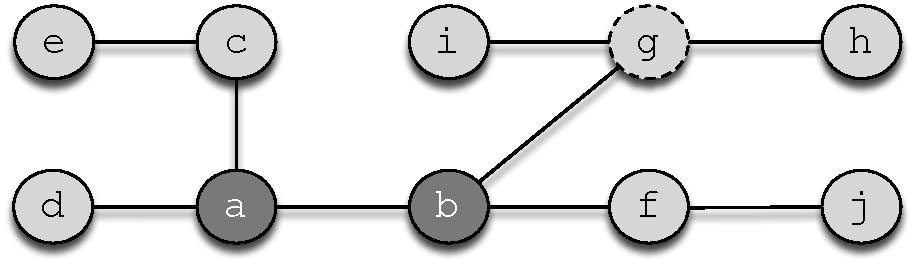
\includegraphics[scale=0.51]{figs/example4.pdf}
%\includegraphics[scale=0.51]{figs/example2.pdf}
\caption{Example power system graph. PMU nodes ($a,b$) are indicated with darker shading. Injection nodes have solid borders while zero-injection nodes  ($g$) have dashed borders.}
\label{fig:example}
\end{figure}

Using the same notation as Brueni and Heath \cite{Brueni05}, we define two $\Gamma$ functions. For $v\in V$ let $\Gamma(v)$ be the set of $v$'s neighbors in $G$, and $\Gamma[v] = \Gamma(v)\cup \{v\}$. 
% Since neighbor relationships are symmetric, $u\in\Gamma(v)\Rightleftarrow v\in\Gamma(u)$. 
A PMU placement $\Phi_G \subseteq V$ is a set of nodes at which PMUs are placed,
%We use the definition of a PMU placement from Brueni and Heath \cite{Brueni05}: a PMU cover, $\Phi$, is a subset of $V$ in which PMUs are placed such that all $v \in V$ and all $(u,v) \in E$ observed.
and $\Phi^R_G\subseteq V$ is the set of observed nodes for graph $G$ with placement $\Phi_G$ (see definition of observability below). %For convenience, we let $\Phi^R$ represent the observed nodes for graph $G$.
$k^* = \min \{|\Phi_G|:\Phi^R_G=V\}$ denotes the minimum number of PMUs needed to observe the entire network. Where the graph $G$ is clear from the context, we drop the $G$ subscript.
%Finally, $m$ is a constant corresponding to a graph $G=(V,E)$ such that $m < |V|$. 

%We let $\Phi^-$ represent the observed edges and $\Phi^R$ represent the observed nodes.
%All notation used in this document is shown in Table \ref{tab:notation}.

For convenience, we refer to any node with a PMU as a \emph{PMU node}. Additionally, for a given PMU placement we say that set $W\subseteq V$ is observed if all nodes in $W$ are observed, and if $W=V$ we refer to the graph as \emph{fully observed}. 


%%%%%%%%%%%%%%%%%%%%%%%%%%%%%%%%%%%%%%%%%%%%%%%%%%%%%%%%%%%%%%%%%%%% BEGIN COMMENT %%%%%%%%%%%%%%%%%%%%%%%%%%%%%%%%%%%%%%%%%%%%%%%%%%%%%%%%%%%%%%%%%%%%%%%%%%%%%%%%%%%%%%%%%%%%%%%%%%%%%%%%%%%%%%%%
\begin{comment}
\begin{table}[t]
\begin{center}
\begin{tabular}{l l} 
\hline \hline
   	{\bf Notation} & {\bf Meaning} \\
		  \hline 
		  	$G$ &  undirected graph $(V,E)$ where each $v \in V$ is a bus and each \\
				&  $(u,v) \in E$ is a transmission line connecting $u$ and $v$\\
			$\Gamma(v)$ & $\{u \in V$ $|$ $(u,v) \in E \}$ \\ 
			$\Gamma[v]$ & $\Gamma(v) \cup \{v\}$ \\
 		 	$n$ & $|V|$ \\
			$\Phi$ & a subset of $V$ in which PMUs are placed such that all \\ 
				   & $v \in V$ and all $(u,v) \in E$ observed  \\
			$\Phi^R$ & set of observed nodes \\
			$\Phi^-$ & set of observed edges \\
			\hline \hline
	\end{tabular}
	\end{center}
\caption{Notation Table}
\label{tab:notation}
\end{table}
\end{comment}
%%%%%%%%%%%%%%%%%%%%%%%%%%%%%%%%%%%%%%%%%%%%%%%%%%%%%%%%%%%%%%%%%%%% END COMMENT %%%%%%%%%%%%%%%%%%%%%%%%%%%%%%%%%%%%%%%%%%%%%%%%%%%%%%%%%%%%%%%%%%%%%%%%%%%%%%%%%%%%%%%%%%%%%%%%%%%%%%%%%%%%%%%%

\subsection{Observability Rules}
\label{subsec:observe}

We use the simplified observability rules elegantly formulated by Brueni and Heath \cite{Brueni05}.  We restate the rules here:  %which we restate here:  %For completeness, we restate the rules here:
%We use the simplified observability rules elegantly stated by Brueni and Heath \cite{Brueni05}, which we restate here:  %For completeness, we restate the rules here:
\begin{enumerate}
	
	\item {\bf Observability Rule 1 (O1)}.  {\it If node $v$ is a PMU node, then $\Gamma[v]$ is observed. Formally, if $v \in \Phi_G$, then $\Gamma[v] \subseteq \Phi^R_G$. }

	\item {\bf Observability Rule 2 (O2)}. {\it If a zero-injection node, $v$, is observed and  $\Gamma(v)\backslash\{u\}$ is observed for some $u\in\Gamma(v)$, then  $\Gamma[v]$ is observed.
	Formally, if $v \in \Phi^R_G \cap V_Z$ and $|\Gamma(v) \cap (V - \Phi^R_G)| \leq 1$, then $\Gamma[v] \subseteq \Phi^R_G$. }

\end{enumerate}

Consider the example in Figure \ref{fig:example}, where the shaded nodes are PMU nodes and $g$ is the only zero-injection node. 
%{\footnote {\small For all power system graphs shown in this document zero-injection nodes have a dashed border and injection nodes have a solid border.}}
Nodes $a-d$ are observed by applying O1 at the PMU at $a$, and nodes $a,b,f$ and $g$ are observed by applying O1 at $b$. 
$e$ cannot be observed via $c$ because $c$ does not have a PMU (O1 does not apply) and is an injection node (O2 does not apply). % so $e$ cannot be observed via $c$, which is its only neighbor. 
%$c$ does not have a PMU (O1 does not apply) and is an injection node (O2 does not apply), so $e$ cannot be observed via $c$, which is its only neighbor. 
Similarly, $j$ is not observed via $f$. Finally, although $g \in V_Z$, O2 cannot be applied at $g$ because $g$ has two unobserved neighbors $i,h$, so they remain unobserved.

Since O2 only applies with zero-injection nodes, more nodes are likely observed when nodes are zero-injection. For example, consider the case where $c$ and $f$ are {\em zero-injection} nodes. $a-d$, $g$ and $f$ are still observed as before, as O1 makes no 
conditions on the node type. Additionally, 
since $c,f \in V_Z$ and each has a single unobserved neighbor,  we can apply O2 at each of them to observe $e,j$, respectively. % making $e$ and $j$, respectively, observed.   
We evaluate the effect of increasing the number of zero-injection nodes on observability in our simulations (Section \ref{subsec:zero}).

%Finally, O2 can be applied at $e$ because $e \in V_Z$, $e$ is observed, and all of $e$'s neighbors except $i$ are observed. As a result, $i$ becomes observed. 
%Note that O2 cannot be applied at $f$ because $f$ has two unobserved neighbors. %This leaves $g$ and $h$ as the only two unobserved nodes in this example. 

%\begin{figure*}[t]
%  \begin{center}
%    \fbox{\subfigure[Case O1]{\label{fig:s1}\includegraphics[scale=0.28]{figs/s1.pdf}}}
%    \fbox{\subfigure[Case O2]{\label{fig:s2}\includegraphics[scale=0.28]{figs/s2.pdf}}} 
%  \end{center}
%	\caption{Rule Set 2} 
%  \label{fig:ruleset2}
%\end{figure*}




\subsection{Cross-Validation Rules}
\label{subsec:xval-rules}

% If phasor measured by 2 or more PMUs
From Vanfretti et al. \cite{Vanfretti10}, PMU measurements can be cross-validated when: (1) a 
voltage phasor of a non-PMU bus can be computed by PMU data from two different buses or (2) the current phasor of a transmission line can be computed from PMU data from two different buses. 
%Note that Vanfretti et al. \cite{Vanfretti10} use the term ``redundancy'' instead of cross-validation.  
{\footnote {\small  Vanfretti et al. \cite{Vanfretti10} use the term ``redundancy'' instead of cross-validation. }}  
Although it is the PMU data that is actually being cross-validated,
for convenience, we say a PMU is cross-validated. 
A PMU is \emph{cross-validated} if one of the rules below is satisfied \cite{Vanfretti10}: 
\begin{enumerate}
	
	\item {\bf Cross-Validation Rule 1 (XV1)}.  {\it If two PMU nodes are adjacent, then the PMUs cross-validate each other. % (Figure \ref{fig:validate}(a)). 
	Formally, if $u, v \in \Phi_G$, $u \in \Gamma(v)$, then the PMUs at $u$ and $v$ are cross-validated.}

	\item {\bf Cross-Validation Rule 2 (XV2)}. {\it If two PMU nodes have a common neighbor, then the PMUs cross-validate each other. % (Figure \ref{fig:validate}(b)). 
	Formally, if $u, v \in \Phi_G$, $u\neq v$ and $\Gamma(u)\cap\Gamma(v)\neq\emptyset$, then the PMUs at $u$ and $v$ are cross-validated.}
\end{enumerate}
In short, the cross-validation rules require that {\em the PMU is within two hops of another PMU}.
For example, in Figure \ref{fig:example}, the PMUs at $a$ and $b$ cross-validate each other by XV1. 

XV1 derives from the fact that both PMUs are measuring the current phasor of the transmission line connecting the two PMU nodes.  XV2 is more subtle.  
Using the notation specified in XV2, when computing the voltage phasor of an element in $\Gamma(u)\cap\Gamma(v)$ the voltage equations include variables to 
account for measurement error (e.g., angle bias) \cite{Vanfretti-thesis}. %\cite{Vanfretti10}.
When the PMUs are two hops from each other, there are more equations than unknowns, allowing for measurement error detection. 
Otherwise, the number of unknown variables exceeds the number of equations, which eliminates the possibility of detecting measurement errors \cite{Vanfretti-thesis}.
%Otherwise, the number of unknown variables grows faster than the number of equations, which eliminates the possibility of detecting measurement errors \cite{Vanfretti-thesis}.

%XV1 derives from the fact that both PMUs are measuring the current phasor of the transmission line connecting the two PMU nodes.  XV2 is more subtle.
%Using the notation specified in XV2, when computing the voltage phasor of an element in $\Gamma(u)\cap\Gamma(v)$ the equations include variables to account for measurement error (e.g., angle bias).
%%In order to account for measurement error, the equations used to compute the voltage phasor of the neighbor node shared by the PMU nodes include varialbes to account
%%for measurement error. Computing the voltage phasor of the neighbor node shared by the two PMU nodes
%%When computing the voltage phasor of the common neighbor node shared by the PMU nodes the equations include variables to account for measurement error (e.g., angle bias).
%When the PMUs are two hops from each other, there are more equations than unknowns, allowing for measurement error detection.
%Otherwise, the number of unknown variables exceeds the number of equations, which eliminates the possibility of detecting measurement errors \cite{Vanfretti-thesis}.
%Otherwise, the number of unknown variables grows faster than the number of equations, which eliminates the possibility of detecting measurement errors \cite{Vanfretti-thesis}.






%\input{problem-stmt-long}
\section{Problem Formulations and NP-Completeness Proofs}
\label{sec:problem-analysis}

In this section we define four PMU placement problems and prove the NP-Completeness of each. We begin with a general overview of NP-Completeness, as well as a high-level description of our proof 
strategy in this paper (Section \ref{subsec:proofstrat}). In the remainder of Section \ref{sec:problem-analysis} we present and prove the NP-Completeness of four PMU placement problems, 
in the following order: \full (Section \ref{subsec:full}), \maxinc (Section \ref{subsec:maxinc}), \xval (Section \ref{subsec:xval}), and \xvalpart (Section \ref{subsec:xvalpart}).

In all four problems defined in this paper, we are only concerned with computing the voltage phasors of each bus (i.e., observing the buses). Using the values of the voltage phasors,
Ohm's Law can be easily applied to compute the current phasors of each transmission line.
Also, we consider networks with both injection and zero-injection buses. For similar proofs for purely zero-injection systems, see our Technical Report \cite{Tech11}.

\subsection{NP-Completeness Overview and Proof Strategy}
\label{subsec:proofstrat}
Before proving that our PMU placement problems are NP-Complete (abbreviated NPC), we provide some background on NP-Completeness. NPC problems are the hardest problems in complexity class $\mathcal{NP}$. 
It is generally assumed that solving NPC problems is hard, meaning that any algorithm that solves an NPC problem has exponential running time as function of the input size. It is important to clarify that despite being NPC, a {\em specific} problem instance might be efficiently solvable. This is either due to the special structure of the specific instance or because the input size is small, yielding a small exponent. 
For example, in Section \ref{sec:simulations} we are able to solve \full for small IEEE bus topologies due to their small size. Thus, by establishing that our PMU placement problems are NPC, we claim that there {\em exist} bus 
topologies for which these problems are difficult to solve (i.e., no known polynomial-time algorithm exists to solve those case).  

To prove our problems are NPC, we follow the standard three-step reduction procedure. For a decision problem $\Pi$, we first show $\Pi\in\mathcal{NP}$. Second, we select a known NPC problem, denoted $\Pi'$,
and construct a polynomial-time transformation, $f$, that maps any instance of $\Pi'$  to an instance of $\Pi$. Finally, we must ensure that for this $f$,  $x\in\Pi'\Leftrightarrow f(x)\in\Pi$ \cite{Garey79}.

Next, we outline the proof strategy we use throughout the paper. In Sections  \ref{subsec:full} through Section \ref{subsec:xvalpart} we use slight variations of the approach presented
by Brueni and Heath in \cite{Brueni05} to prove the problems we consider here are NPC. In general we found their scheme to be elegantly extensible for proving many properties of PMU placements.
%For purposes of clarity, we begin by explaining this approach in general terms, and then consider the approach in detail for each problem.

In \cite{Brueni05}, the authors prove NP-Completeness by reduction from planar 3-SAT (\sats). A 3-SAT formula, $\phi$, is a boolean formula in conjunctive normal form (CNF) such that each clause contains at most $3$ literals. For any 3-SAT formula $\phi$ with the sets of variables $\{v_1,v_2, \dots , v_r\}$ and clauses $\{c_1,c_2, \dots , c_s \}$, $G(\phi)$ is the bipartite graph $G(\phi)=(V(\phi),E(\phi))$ defined as follows:
\begin{eqnarray*}
% \nonumber to remove numbering (before each equation)
 V(\phi) &= &\{v_i\; \vert\; 1 \leq i \leq r \} \cup \{c_j \;\vert\; 1 \leq j \leq s \} \\
 E(\phi) &=& \{ (v_i,c_j)\;\vert\; v_i \in c_j\;\; or \;\; \overline{v_i} \in c_j\}.
\end{eqnarray*}
Note that edges pass only between $v$ and $c$ nodes, and so the graph is bipartite.  \sat is a 3-SAT formula s.t.  $G(\phi)$ is planar \cite{Lich82}. For example, \sat formula
\begin{eqnarray}
	 \varphi &=& (\overline{v_1} \vee v_2 \vee v_3) \wedge (\overline{v_1} \vee \overline{v_4} \vee v_5) \wedge (\overline{v_2} \vee \overline{v_3} \vee \overline{v_5}) \nonumber\\
	 & & \wedge (v_3 \vee \overline{v_4}) \wedge  (\overline{v_3} \vee v_4 \vee \overline{v_5})
\label{eqn:varphi}
\end{eqnarray}
has graph $G(\varphi)$ shown in Figure \ref{fig:gvarphi}. Discovering a satisfying assignment for  \sat is an NPC problem, and so it can be used in a reduction to prove the complexity of the problems we address here. Note that in this work we will use $\varphi$ to denote a specific \sat formula, while $\phi$ will be used to denote a generic \sat formula.

Following the approach in \cite{Brueni05}, for \sat formula, $\phi$, we replace each variable node and each clause node in $G(\phi)$ with a specially constructed set of nodes,
termed a {\em gadget}. In this work, all variable gadgets will have the same structure, and all clause gadgets have the same structure (that is different from the variable gadget structure), and we denote the resulting graph as $H(\phi)$.
In $H(\phi)$, each {\em variable} gadget has a subset of nodes that semantically represent assigning ``True" to that variable, and a subset of nodes that represent assigning it ``False". When a PMU is placed at one of these nodes, this is interpreted as assigning 
a truth value to the \sat variable corresponding with that gadget. 
Thus, we use the PMU placement to determine a consistent truth value for each \sat variable. 
%Reading variable assignments off such a network with PMUs requires that each variable get a consistent truth value via PMU placements. 
Also, clause gadgets are connected to variable gadgets at either ``True" or ``False" (but never both) nodes, in such a way that the clause is satisfied if and only if {\em at least one} of those nodes has a PMU.

We also note that while we assume $G(\phi)$ is planar, we make no such claim regarding $H(\phi)$, though in practice all graphs used in our proofs are indeed planar. The proof of NPC rests on the fact that solving the underlying $\phi$ formula is NPC.

In what follows, for a given PMU placement problem $\Pi$, we prove $\Pi$ is NPC by showing that a PMU placement in $H(\phi)$, $\Phi$, can be interpreted semantically as describing a satisfying assignment for $\phi$ iff $\Phi\in\Pi$. 
Since \sat is NPC, this proves $\Pi$ is  NPC as well.

%the problem exactly. NP-Complete problems are the hardest problem in completixty class $\mathcal{P}$.  Showing a problem is NP-Complete is a two step procedure: (1) show that a solution
%to the problem can be verified in polynomial time and (2) all known NP-Complete problems are at least as hard as $L$.  Step (2) is done through a reduction: .

\begin{figure}[t]
\centering
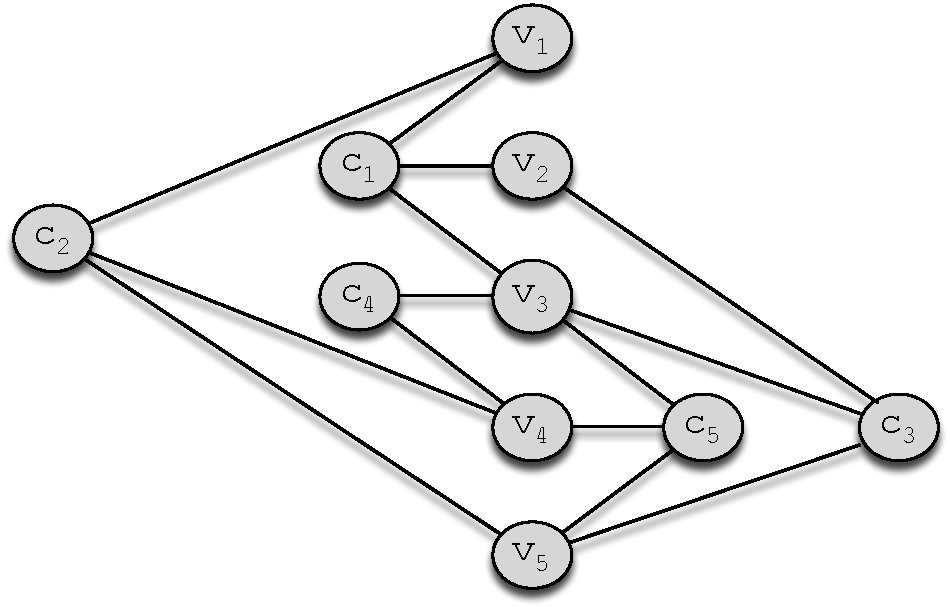
\includegraphics[scale=0.53]{figs/gvarphi.pdf}
\caption{$G(\varphi)=(V(\varphi),E(\varphi))$ formed from $\varphi$ in Equation (\ref{eqn:varphi}) }
\label{fig:gvarphi}
\end{figure}


\subsection{The \full Problem}
\label{subsec:full}

%\begin{figure}[t]
%\centering
%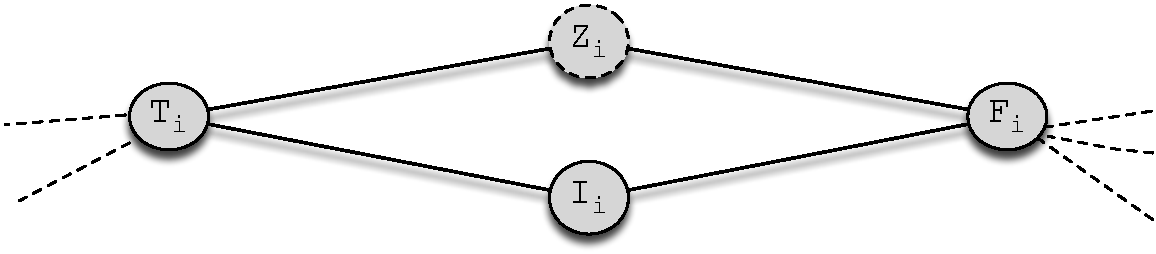
\includegraphics[scale=0.43]{figs/diamond-gadget.pdf}
%\caption{Variable gadget used in Theorem \ref{thm:npc-full}. $Z_i$ is a zero-injection node and all other nodes are injection nodes.}
%\label{fig:diamond-gadget}
%\end{figure}

\begin{figure}[t]
 % \begin{center}
    \fbox{\subfigure[Variable gadget $V_i$ used in Theorem \ref{thm:npc-full} and Theorem \ref{thm:npc-maxinc}. The dashed edges are connections to clause gadgets. $Z_i$ is a zero-injection node and all other nodes are injection nodes.]
	{\label{fig:diamond-gadget}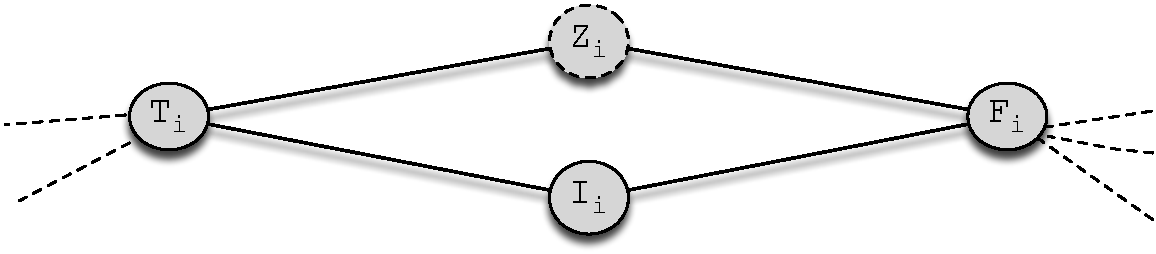
\includegraphics[scale=0.29]{figs/diamond-gadget.pdf}}}
    \fbox{\subfigure[Clause gadget $C_j$ used in Theorem \ref{thm:npc-maxinc}. The dashed edges are connections to variable gadgets. $a_j$ and $b_j$ are both injection nodes.]{\label{fig:line-gadget}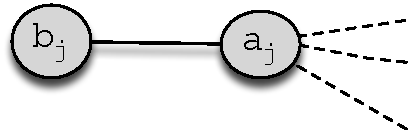
\includegraphics[scale=0.29]{figs/line-gadget.pdf}}}
  %\end{center}
	\caption{Gadgets used in  Theorem \ref{thm:npc-full} and Theorem \ref{thm:npc-maxinc}.}
  \label{fig:maxinc}
\end{figure}



The \full problem was previously discussed in the literature (e.g., the PMUP problem in \cite{Brueni05}, and the PDS problem in \cite{Haynes02}) for purely zero-injection bus systems. Here we consider networks with mixtures of injection and zero-injection buses, and modify the NPC proof for PMUP in \cite{Brueni05} to handle this mixture.

\full Optimization Problem:
\begin{itemize}
	\item \underline{Input}: Graph $G=(V,E)$ where $V=V_Z \cup V_I$ and $V_Z \neq \emptyset$.
	{\footnote {\small We include the condition that $V_Z \neq \emptyset$ because otherwise \full reduces to \textsc{Vertex-Cover}, making the NP-Completeness
	proof trivial.}}

	\item \underline{Output}: A placement of PMUs, $\Phi_G$, such that $\Phi^R_G=V$ and $\Phi_G$ is minimal.
	%\textsc{Output}: A placement of $k$ PMUs, $\Phi$, such that $|\Phi^R|$ is maximal.
\end{itemize}

\full Decision Problem:
\begin{itemize}
	\item \underline{Instance}: Graph $G=(V,E)$ where $V=V_Z \cup V_I$, $V_Z \neq \emptyset$, $k$ PMUs such that $k \geq 1$.

	\item \underline{Question}: Is there a $\Phi_G$ such that $|\Phi_G| \leq k$ and $\Phi^R_G = V$?
	%\item \underline{Question}: Is there a $\Phi \subseteq V$ such that $|\Phi| \leq k$ and $m \leq |\Phi^R| < |V|$?
\end{itemize}

%The corresponding {\em optimization problem} is to find the minimal value $k$ such that the entire network is observed. It is well-known that these two formulations are equivalent complexity-wise, 
%and thus we present and prove only the complexity of the decision problem here. A formal definition of the optimization problem can be found in the technical report \xxx{CITE}. 

\begin{theorem}
\full is NP-Complete. %even when restricted to the class of bipartite planar graphs.
\label{thm:npc-full}
\end{theorem}

{\bf Proof Idea}:  We introduce a problem-specific variable gadget. We show that in order to observe all nodes, PMUs must be placed on variable gadgets, specifically on
nodes that semantically correspond to True and False values that satisfy the corresponding \sat formula. 

For our first problem, we use a single node as a clause gadget denoted $a_j$, and the subgraph shown in Figure \ref{fig:diamond-gadget} as the variable gadget. Note that in the variable gadget, all the nodes are injection nodes except for $Z_i$. For this subgraph, we state the following simple lemma:

\begin{lemma}\label{lem:property1}
Consider the gadget shown in Figure \ref{fig:diamond-gadget}, possibly with additional edges connected to $T_i$ and/or $F_i$. Then (a) nodes $I_i, Z_i$ are not observed if there is no PMU on the gadget, and (b) all the nodes in the gadget are observed with a single PMU iff the PMU is placed on either $T_i$ or $F_i$.
\end{lemma}
\begin{proof}
(a) If there is no PMU on the gadget, O1 cannot be applied at any of the nodes, and so we must resort to O2. We assume no edges connected to $I_i,Z_i$ from outside the gadget, and since $T_i,F_i\in V_I$, we cannot apply O2 at them, which concludes our proof.
 
(b) In one direction, if we have a PMU placed at $T_i$, from O1 we can observe $Z_i,I_i$. Since $Z_i$ is zero-injection and one neighbor, $T_i$ has been observed, from O2 at $Z_i$ we can observe $F_i$. The same holds for placing a PMU at $F_i$, due to symmetry.

In the other direction, by placing a PMU at $I_i$ ($Z_i$) we observe $T_i$ and $F_i$ via O1. However, since $F_i,T_i\notin V_Z$, O2 cannot be applied at either of them, so $Z_i$ ($I_i$) will not be observed. \qed
\end{proof}

\begin{proof}[of Theorem \ref{thm:npc-full}]
%\maxinc is easily in $\in \mathcal{NP}$.
We start by arguing that \full $\in \mathcal{NP}$. First, nondeterministically select $k$ nodes in which to place PMUs. Using the rules specified in Section \ref{subsec:observe}, determining
the number of observed nodes can be done in linear time.
%Haynes et al. \cite{Haynes02} show that given a PDS solution can be verified in polynomial time. Since \maxinc only checks $m < |V|$ vertices,
%the same algorithm can be used to verify a \maxinc solution in polynomial time.

To show \full is NP-hard, we reduce from \sats.  Let $\phi$ be an arbitrary \sat formula with variables 
$\{v_1,v_2, \dots , v_r\}$ and the set of clauses $\{c_1,c_2,\dots , c_s \}$, and $G(\phi)$ the corresponding planar graph. We use $G(\phi)$ to construct a new graph $H_0(\phi) = (V_0(\phi), E_0(\phi))$ by replacing each variable
node in $G(\phi)$ with the variable gadget shown in Figure \ref{fig:diamond-gadget}. The clause nodes consist of a single node (i.e., are the same
as in $G(\phi)$). We denote the node corresponding to $c_j$ as $a_j$. All clause nodes are injection nodes.  In the remainder of this proof we let $H := H_0(\phi)$.
In total, $V_Z$ contains all $Z_i$ nodes for $1 \leq i \leq r$, and all other nodes are in $V_I$.  The edges connecting clause nodes with variable gadgets express which variables are in each clause: for each clause node $a_j$, $(T_i, a_j)\in E_0(\phi) \Leftrightarrow v_i\in c_j$, and $(F_i, a_j)\in E_0(\phi) \Leftrightarrow \overline{v_i}\in c_j$. As a result, the following observation holds:

\begin{observation}\label{obs:1}
For a given truth assignment and a corresponding PMU placement, a clause $c_j$ is satisfied iff $a_j$ is attached to a node in a variable gadget with a PMU. 
\end{observation}


The resulting graph for the example given in Figure \ref{fig:gvarphi} is shown in Figure \ref{fig:proof1-inject-example}.  Nodes with a dashed border are zero-injection nodes. 
{\footnote {\small  Throughout this paper, nodes with dashed borders denote zero-injection nodes. }} 
The corresponding formula for this graph, $\varphi$,
is satisfied by truth assignment $A_{\varphi}$: $\overline{v_1}, \overline{v_2}, v_3, \overline{v_4},$ and $\overline{v_5}$ are True. This corresponds to the dark shaded nodes in Figure
\ref{fig:proof1-inject-example}. While this construction generates a graph with very specific structure, in Section \ref{subsec:extend}, we detail how to extend our proof to consider graphs with a wider range of structures.% different $\frac{|V_Z|}{|V_I|}$ ratios.


With this construct in place, we move on to our proof. We show that $\phi$ is satisfiable if and only if $k=r=|\Phi_H|$ PMUs
can be placed on $H$ such that $\Phi^R_{H}=V$.

$(\Rightarrow)$ Assume $\phi$ is satisfiable by truth assignment $A_{\phi}$. Then, consider the placement $\Phi_H$ such that for each variable gadget $V_i$, $T_i\in \Phi_H \Leftrightarrow v_i=True$
in $A_\phi$, and  $F_i\in \Phi_H \Leftrightarrow v_i=False$. From Lemma \ref{lem:property1}(b) we know that all nodes in variable gadgets are observed by such a placement. From Observation \ref{obs:1}, all clause nodes are observed because our PMU assignment is based on a satisfying assignment.
Thus, we have shown that $\Phi^R_{H}=V$.

$(\Leftarrow)$
Suppose there is a placement of $r$ PMUs, $\Phi_H$, such that $\Phi_H^R = V$.  From Lemma \ref{lem:property1}(a) we know that for each $V_i$ with no PMU, at least two nodes are not observed, so each $V_i$  must have a PMU placed in it. 
Since we have only $r$ PMUs, that means one PMU per gadget. From Lemma \ref{lem:property1}(b) we know this PMU must be placed on $T_i$ or $F_i$, since otherwise the gadget will not be fully observed. Note that these nodes are all in $V_I$.

Since we assume the graph is fully observed, all $a_j$ are observed by $\Phi_H$. Because we just concluded that PMUs are placed only on injection nodes in the variable gadgets, each clause node $a_j$ can only be observed via application of O1 at $T_i/F_i$ nodes to which it is attached -- specifically, $a_j$ is attached to a node with a PMU. From Observation \ref{obs:1} this means that all clauses are satisfied by the semantic interpretation of our PMU placement, which concludes our proof. \qed

%Because each clause node, $a_j$, is only connected to $T_i$ or $F_i$ nodes of each variable gadget, $V_i$, and $T_i,F_i \notin V_Z$, each $a_j$ must be observed by applying O1 at an adjacent $T_i$ or $F_i$ node.  Therefore, by assigning
%each $v_i \in \phi$ to $True$ iff $T_i \in \Phi_G$ and each $v_i \in \phi$ to $False$ iff $F_i \in \Phi_G$, we can derive a satisfying truth assignment for $\phi$ from $\Phi_G$. \qed

%Because the $T_i$ and $F_i$ nodes of each variable gadget are connected to clause nodes in exactly the same manner as the $T$ and $F$ variable gadget nodes in \cite{Brueni05},
%we use the proof in \cite{Brueni05} to determine that all clauses in $\phi$ are satisfied by the truth assignment derived from $\Phi_G$. \qed
\end{proof}



\subsection{The \maxinc Problem}
\label{subsec:maxinc}

%Here we define both an optimization and decision version of the \maxinc problem.
\maxinc is a variation of \fulls: rather than consider the minimum number of PMUs required for full system observability,
\maxinc finds the maximum number of nodes that can be observed using a fixed number of PMUs.

%Before formally stating the \maxinc problem, we present some notation.
%Let $k^*$ be the minimum number of PMUs needed for $\Phi^R = V$. Let $\Phi^R_G$ and $\Phi^R_{G'}$ be the observed nodes for graph $G$ and $G'$, respectively. Finally, $m$ is a
%constant corresponding to a graph $G=(V,E)$ such that $m < |V|$.

\maxinc Optimization Problem:
\begin{itemize}
	%\textsc{Input}: Graph $G=(V,E)$, $k$ PMUs such that $1 \leq k < k^*$.
	\item \underline{Input}: Graph $G=(V,E)$ where $V=V_Z \cup V_I$, $k$ PMUs such that $1 \leq k < k^*$.

	\item \underline{Output}: A placement of $k$ PMUs, $\Phi_G$, such that $|\Phi^R_G|$ is maximum.
%	%\textsc{Output}: A placement of $k$ PMUs, $\Phi$, such that $|\Phi^R|$ is maximal.
\end{itemize}

\maxinc Decision Problem:
\begin{itemize}
	\item \underline{Instance}: Graph $G=(V,E)$ where $V=V_Z \cup V_I$, $k$ PMUs such that $1 \leq k < k^*$.

	\item \underline{Question}: For a given $m< |V|$, is there a $\Phi_G$ such that $|\Phi_G| \leq k$ and $m \leq |\Phi^R_G| < |V|$?
	%\item \underline{Question}: Is there a $\Phi \subseteq V$ such that $|\Phi| \leq k$ and $m \leq |\Phi^R| < |V|$?
\end{itemize}

%The corresponding {\em optimization problem} is to find the maximal value $m$ for the given network and $k$ PMUs. A formal definition of the optimization problem can be found in the technical report \xxx{CITE}. 


\begin{figure}[t]
\centering
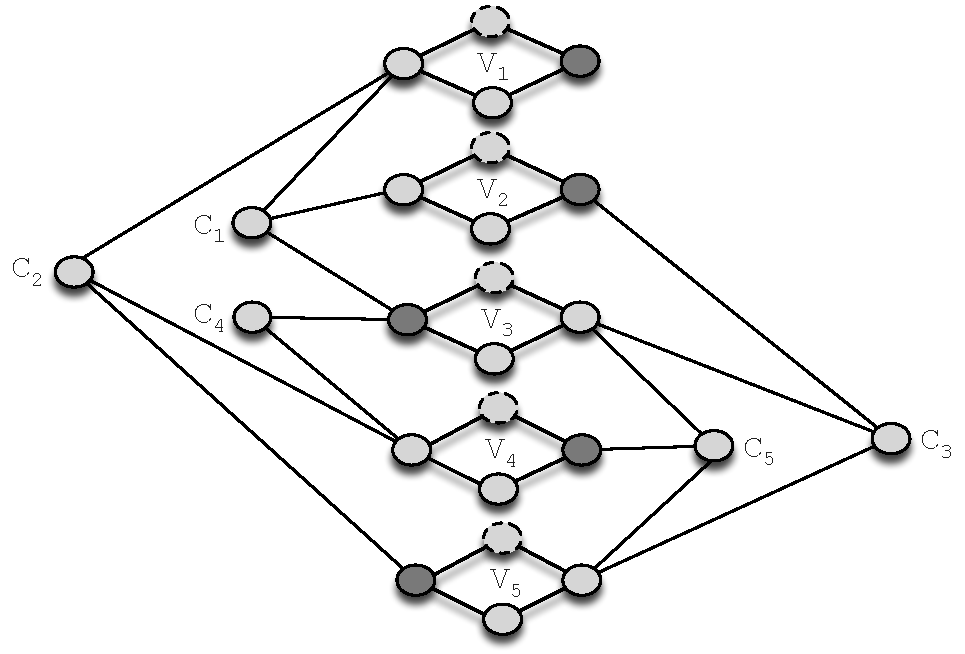
\includegraphics[scale=0.53]{figs/proof1-inject-example.pdf}
%\includegraphics[scale=0.51]{figs/example2.pdf}
\caption{Graph $G=(V,E)=H_1(\varphi)$ formed from $\varphi$ formula in Theorem \ref{thm:npc-full} proof. Nodes with a dashed border are zero-injection nodes.}
\label{fig:proof1-inject-example}
\end{figure}

\begin{theorem}
\maxinc is NP-Complete. %even when restricted to the class of bipartite planar graphs.
\label{thm:npc-maxinc}
\end{theorem}

{\bf Proof Idea}: First, we construct problem-specific gadgets for variables and clauses. We then demonstrate that any solution that observes $m$ nodes must place the PMUs only on nodes
in the variable gadgets. Next we show that as a result of this, the problem of observing $m$ nodes in this graph reduces to Theorem \ref{thm:npc-full}.

\begin{proof}
%\maxinc is easily in $\in \mathcal{NP}$.
\maxinc $\in \mathcal{NP}$ using the same argument in the proof for Theorem \ref{thm:npc-full}.

Next, we reduce from {\sat} as in the proof for Theorem \ref{thm:npc-full}, where $\phi$ is an arbitrary \sat formula. We create a new graph $H_1(\phi) = (V_1(\phi), E_1(\phi))$ which is identical to $H_0(\phi)$ from the previous proof, except that each clause node in $H_0(\phi)$ is replaced with the clause gadget shown in Figure \ref{fig:line-gadget}, comprising of two injection nodes. As before, the edges connecting clause nodes with variable gadgets express which variables are in each clause: for each clause node $a_j$, $(T_i, a_j)\in E_1(\phi) \Leftrightarrow v_i\in c_j$, and $(F_i, a_j)\in E_1(\phi) \Leftrightarrow \overline{v_i}\in c_j$. Note that Observation \ref{obs:1} holds here as well.



% Before beginning our proof that \maxinc is NP-hard, we briefly summarize the reduction from \sat used in \cite{Brueni05}.
% Given a \sat formula, $\phi$, with variables $\{v_1,v_2, \dots , v_r\}$ and the set of
% clauses $\{c_1,c_2, \dots , c_s \}$, a graph $H(\phi) = (V(\phi),E(\phi))$ is formed as follows.  Each variable, $v_i$, is replaced with a gadget shown in Figure \ref{fig:variable-gadget}.  Each
% clause, $c_j$, is replaced with a 2-clique $C[j],C'[j]$.  The edges in $E(\phi)$ represent whether a clause contains a variable.  If the variable $v_i$ occurs in clause $c_j$, $C[j]$ is connected to
% $v_i$'s $T$ node. Conversely, if $\overline{v_i}$ occurs in clause $c_j$, then $C[j]$ is connected to $v_i$'s $F$ node.
% Figure \ref{fig:proof1-example} shows the graph $H(\varphi)$ formed from \sat formula $\varphi$, defined in Equation (\ref{eqn:varphi}), with one exception:
% for each clause gadget, $C_j$, $C_j$'s two leaf nodes are removed.

% In our proof, we define the same \sat formula, $\phi$, as in \cite{Brueni05}: $\phi$ has variables $\{v_1,v_2, \dots , v_r\}$ and the set of clauses $\{c_1,c_2, \dots , c_s \}$.
% From $\phi$, we create a graph $G=(V,E)$ which is identical to $H(\phi)$ defined in \cite{Brueni05} with one exception. We replace each 2-clique $\{C[j],C'[j]\} \in H(\phi)$ with
% clause gadget $C_j$. Each $C_j$ has the following $\Gamma$ functions: $\Gamma(d_j) = \{b_j\}$, $\Gamma(e_j) = \{b_j\}$, $\Gamma(b_j) = \{a_j,d_j,e_j\}$, and $\Gamma(a_j) = \Gamma_o(C[j]) \cup \{b_j\}$
% where $\Gamma_o(C[j])$ is the $\Gamma$ function for $C[j] \in H(\phi)$. $C_j$ is shown in Figure \ref{fig:clause-gadget}.

% For example, the graph for formula $\varphi$ defined in Equation (\ref{eqn:varphi}) is shown in Figure \ref{fig:proof1-example}.
% $\varphi$ is satisfied by truth assignment $A_{\varphi}$: $\overline{v_1}, \overline{v_2}, v_3, \overline{v_4},$ and $\overline{v_5}$ are true.
% The dark shaded nodes have PMUs and correspond to $A_{\varphi}$.

We are now ready to show \maxinc is NP-hard. For convenience, we let $H := H_1(\phi)$.  Recall $\phi$ has $r$ variables and $s$ clauses. 
Here we consider the instance of \maxinc where $k=r$ and $m = 4r + s$, and show that $\phi$ is satisfiable if and only if $r=|\Phi_H|$ PMUs
can be placed on $H$ such that $m \leq |\Phi^R_{H}| < |V|$. In Section \ref{subsec:extend} we discuss how to extend this proof for any larger value of $m$ and different $\frac{|V_Z|}{|V_I|}$ ratios.

$(\Rightarrow)$ Assume $\phi$ is satisfiable by truth assignment $A_{\phi}$. Then, consider the placement $\Phi_H$ such that for each variable gadget $V_i$, $T_i\in \Phi_H \Leftrightarrow v_i=True$
in $A_\phi$, and  $F_i\in \Phi_H \Leftrightarrow v_i=False$.  In the proof for Theorem \ref{thm:npc-full} we demonstrated such a placement will observe all nodes in $H_0(\phi)\subset H_1(\phi)$, and using the same argument it can easily be checked that these nodes are still observed in $H_1(\phi)$. Each $b_j$ node remains unobserved because each $a_j \in V_I$ and consequently O2 cannot be applied at $a_j$.
Since $|H_0(\phi)|=4r+s = m$, we have observed the required nodes.

$(\Leftarrow)$
We begin by proving that any solution that observes $m$ nodes must place the PMUs only on nodes in the variable gadgets. By construction, each PMU is either on a clause gadget or a variable gadget, but not both. Let $0\leq t\leq r$ be the number of PMUs on clause gadgets, we wish to show that for the given placement $t=0$. First, note that {\em at least} $\max(s-t,0)$ clause gadgets are without PMUs, and that for each such clause (by construction) at least one node ($b_i$) is not observed. Next, from Lemma \ref{lem:property1}(a) we know that for each variable gadget without a PMU, at least two nodes are not observed.

Denote the {\em unobserved} nodes for a given PMU placement as $\Phi_H^-$. Thus, we get $|\Phi_H^-| \geq 2t + \max((s-t), 0)$. However, since $m$ nodes are observed and  $|V|-m \leq s$, we get $|\Phi_H^-| \leq s$, so we know $s \geq 2t + \max((s-t), 0)$. We consider two cases:
\begin{itemize}
	\item $s\geq t$: then we get $s \geq t + s \Rightarrow t=0.$
	\item $s < t$:	then we get $s \geq 2t$, and since we assume here $0\leq s < t$ this leads to a contradiction and so this case cannot occur.
\end{itemize}

Thus, the $r$ PMUs must be on nodes in variable gadgets. Note that the variable gadgets in $H_1(\phi)$ have the same structure as in $H_0(\phi)$. We return to this point shortly.

Earlier we noted that for each clause gadget without a PMU, the corresponding $b_j$ node is unobserved, which comes to $s$ nodes. To observe $m=4r+s$ nodes, we will need to observe all the remaining nodes. Thus, we have reduced the problem to that of observing all of $H_0(\phi)\subset H_1(\phi)$. Our proof for Theorem \ref{thm:npc-full} demonstrated this can only be done by placing PMUs at nodes corresponding to a satisfying assignment of $\phi$, and so our proof is complete. \qed
\end{proof}
%Finally, we show that $G$ is bipartite and planar. From \cite{Brueni05} we know that $H(\phi)$ is bipartite and planar.  Recall, the only difference between $G$ and $H(\phi)$ is that $G$'s clause
%gadgets have two extra nodes: $d_j$ and $e_j$.  We must show that the addition of all $d_j$ and $e_j$ to $H(\phi)$ maintains the condition that the resulting graph, $G$, is bipartite and planar.
%We add $d_j$ and $e_j$ to the same partition as $a_j$, $V_1$.
%Because $d_j$ and $e_j$ are only connected to $b_j$ and $b_j \notin V_1$,
%this maintains the condition that $G$ is bipartite.

%By definition every \sat formula, $\phi$, has a planar embedding $G(\phi)$.  From \cite{Brueni05} we know that $H(\phi)$ maintains the planar
%embedding. By inspection, adding $d_j$ and $e_j$ to $H(\phi)$ preserves the condition that $G$ is planar.
%\end{proof}


\subsection{The \xval Problem}
\label{subsec:xval}

%First we dedine \xval as an optimization problem and then state then state the \xval as a decision problem.

\xval Optimization Problem:
\begin{itemize}
	\item \underline{Input}: Graph $G=(V,E)$ where $V=V_Z \cup V_I$.

	\item \underline{Output}: A placement of PMUs, $\Phi_G$, such that $\Phi^R_G = V$,
	and  $\Phi_G$ is minimal under the condition that each $v \in \Phi_G$ is cross-validated according to the rules specified in Section \ref{subsec:xval}.
\end{itemize}

\xval Decision Problem:
\begin{itemize}
	\item \underline{Instance}: Graph $G=(V,E)$ where $V=V_Z \cup V_I$, $k$ PMUs such that $k \geq 1$.

	\item \underline{Question}: Is there a $\Phi_G$ such that $|\Phi_G| \leq k$ and $\Phi^R_G = V$ under the condition that each $v \in \Phi_G$ is cross-validated?
	%\item \underline{Question}: Is there a $\Phi_G$ such that $|\Phi_G| \leq k$, $\Phi^R_G = V$, and each $v \in \Phi_G$ is cross-validated?
	%\item \underline{Question}: Is there a $\Phi \subseteq V$ such that $|\Phi| \leq k$, $\Phi^R = V$, and each $\phi \in \Phi$ is cross-validated?
\end{itemize}

%The corresponding {\em optimization problem} is to find the minimal $k$ such that the entire network is observed and all PMUs are cross-validated. A formal definition of the optimization problem can be found in the technical report \xxx{CITE}. 

\begin{figure}[t]
\centering
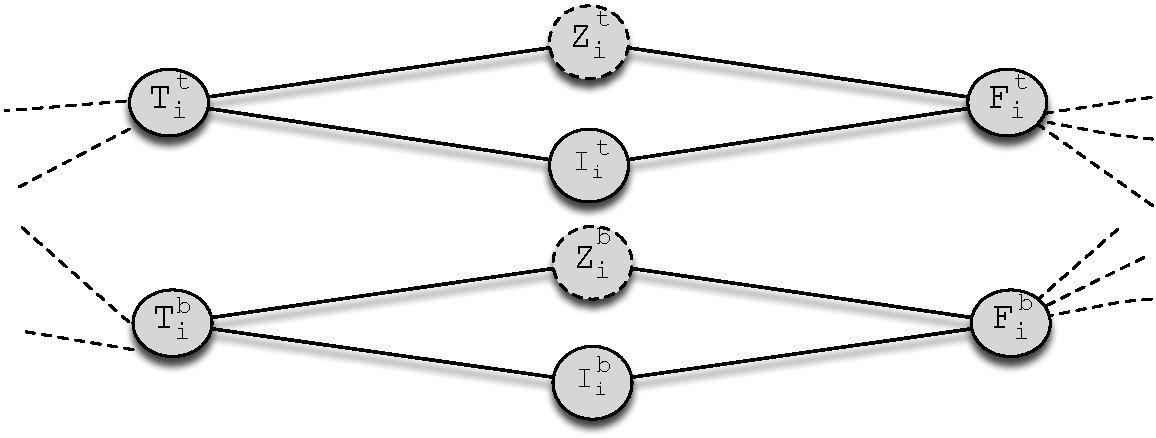
\includegraphics[scale=0.46]{figs/vgadget-inject.pdf}
%\includegraphics[scale=0.51]{figs/example2.pdf}
\caption{Variable gadget used in Theorem \ref{thm:npc-xval} proof.  The gadget has two disconnected subgraphs, where the superscript, $t$, denotes nodes in the upper subgraph and superscript, $b$, indexes
nodes in the lower subgraph. The dashed edges are connections to clause gadgets.}
\label{fig:xval-gadget}
\end{figure}

\begin{theorem}
\xval is NP-Complete. % even when restricted to the class of bipartite and chordal graphs.
\label{thm:npc-xval}
\end{theorem}

% {\bf Proof idea:} We show \xval is NP-hard by reducing from \sats.  Similar to our redcution
% for \maxincs, we create a clause gadget for each clause in \sat forumula, $\phi$, and a variable gadget
% for each variable in $\phi$.  The clause gadget is a pair of nodes connected by an edge.  The variable
% gadget is shown in Figure \ref{fig:xval-gadget}.  A variable gadget, $V_i$, is connected to the clause gadgets, $C_j$, only if
% variable $v_i$ appears in clause $c_i$ in $\phi$.
%
% %If a variable, $v_i$, appears in clause, $c_j$,
% %$c_j$'s clause gadget has the edges $(C[j], T_t), (C[j],T_b)$. Similarily, if clause $c_j$
% %contains variable $\overline{v_i}$ in $\phi$, the $c_j$'s clause gadget has the edges $(C[j], F_t), (C[j],
% %F_b)$.
%
% We place PMUs on variable gadget nodes $T$ and $F$ according to the literal value of each variable in the satisfying truth assignment for $\phi$.
% %PMUs at $T$ nodes are cross-validated using XV2 via the common clause node.
% This leads to a fully observed graph in which all PMUs are cross-validated.  In the other direction, we show that $G$ can only be fully observed
% if $2$ PMUs are placed on each variable gadget. Specifcally, PMUs must be placed on both $T$ nodes or both $F$ nodes, in each variable gadget.  We use the PMU placement
% to derive a satisfying truth assignment for \sat formula $\phi$.
%All clause nodes are observed because each clause is adjacent to at least one PMU node.  The variable clauses are
%Given a satisfying truth assingment to $\phi$, we place PMUs $T$ nodes and $F$ nodes only.
%If a variable $v_i \in \phi$ is True, we place a PMU on each of the $T$ nodes of $v_i$ corresponding variable gadget.  Likewise,
%if $v_i$ is false, a PMU is placed on the $F$ nodes of $v_i$'s variable gadget.

% variable gadgets and clause gadgets
% => place PMUs on T/F nodes of each variable gadget
% <= in order for G to be fully observed each variable gadget must have 2 PMUs,  in order to satisfy cross-validation
%   must be on T/F nodes.  PMU on T node implies variable is true and vice versa.  in this way we derive a satisfying assignment for $\phi$
%

{\bf Proof Idea:}   We show \xval is NP-hard by reducing from \sats.  
We create a single-node gadget for clauses (as for \fulls) and the gadget shown in Figure \ref{fig:xval-gadget} for each variable. Each variable gadget here comprises of two disconnected components, 
and there are two $T_i$ and two $F_i$ nodes, one in each component. First, we show that each variable gadget must have $2$ PMUs for the entire graph to be observed, one PMU for each subgraph.
Then, we show that cross-validation constraints force PMUs to be placed on both $T$ nodes or both $F$ nodes.  Finally, we show how to use the PMU placement to derive a satisfying \sat truth assignment.
 
%Our proof makes use of the following Lemma.  Note that for each variable gadget $V_i$, we refer to the upper subgraph as $V_{i}^t$ and the
%lower subgraph as $V_{i}^b$.

\begin{lemma}\label{lem:property2}
Consider the gadget shown in Figure \ref{fig:xval-gadget}, possibly with additional nodes attached to $T_i$ and/or $F_i$ nodes. (a) nodes $I^t_i, Z^t_i$ are not observed if there is no PMU on $V_i^t$, and (b) all the nodes in $V_i^t$ are observed with a single PMU iff the PMU is placed on either $T_i^t$ or $F_i^t$. Due to symmetry, the same holds when considering $V_i^b$.
\end{lemma}
\begin{proof}
The proof is straightforward from the proof of Lemma \ref{lem:property1}, since both $V_i^t$ and $V_i^b$ are identical to the gadget from Figure \ref{fig:diamond-gadget},  which Lemma \ref{lem:property1} refers to. \qed
\end{proof}

\begin{proof}[of Theorem \ref{thm:npc-xval}]
First, we argue that \xval $\in \mathcal{NP}$.  Given a \xval solution, we use
the polynomial time algorithm described in our proof for Theorem
\ref{thm:npc-full} to determine if all nodes are observed.  Then, for each
PMU node we run a breadth-first search, stopping at depth $2$, to check that
the cross-validation rules are satisfied.

To show \xval is NP-hard, we reduce from \sats.  Our reduction is similar to
the one used in Theorem \ref{thm:npc-full}.  We start with the same \sat formula $\phi$ with variables $\{v_1,v_2, \dots , v_r\}$ and the set of clauses $\{c_1,c_2,\dots , c_s \}$.

% Given a \sat formula, $\phi$,
% with variables $\{v_1,v_2, \dots , v_r\}$ and the set of clauses $\{c_1,c_2,
% \dots , c_s \}$, we form a new graph, $G=(V,E)$, as follows. Each clause $c_j$
% corresponds to a pair of nodes connected by an edge, denoted $C[j],C'[j]$. This
% is the same construct as described in the original proof \cite{Brueni05}.
For this problem, we construct $H_2(\phi)$ in the following manner. We use the single-node clause gadgets  as in $H_0(\phi)$, and as before, the edges connecting clause nodes with variable gadgets shown in Figure \ref{fig:xval-gadget} express which variables are in each clause: for each clause node $a_j$, $(T^t_i, a_j),(T^b_i, a_j)\in E_1(\phi) \Leftrightarrow v_i\in c_j$, and $(F^t_i, a_j),(F^b_i, a_j)\in E_1(\phi) \Leftrightarrow \overline{v_i}\in c_j$. For notational simplicity, we shall use $H$ to refer to $H_2(\phi)$. Note that once again, by construction Observation \ref{obs:1} holds for $H$.

%Let $k = 2r$.
Moving on, we now show that $\phi$ is satisfiable if and only if
$k=2r$ PMUs can be placed on $H$ such that $H$ is fully observed under the
condition that all PMUs are cross-validated, and that $2r$ PMUs are the minimal
bound for observing the graph with cross-validation.

$(\Rightarrow)$ Assume $\phi$ is satisfiable by truth assignment $A_{\phi}$.
For each $1\leq i\leq r$, if $v_i=True$ in $A_{\phi}$ we place a PMU at $T_i^b$
and at $T_i^t$ of the variable gadget $V_i$. Otherwise, we place a PMU at $F_i^b$
and at $F_i^t$ of this gadget. From the fact that $A_{\phi}$ is satisfying and Observation \ref{obs:1}, we know the PMU nodes in $V_i$ must be
adjacent to some clause node\footnote{Each variable must be used in at least a single clause, or it is not considered part of the formula. If there is a variable that has no impact on the truth value of $\phi$, we always place the PMUs on two nodes (both T or both F) that are adjacent to a clause node.}, making $T_i^t$ ($F_i^t$) two hops away from
$T_i^b$ ($F_i^b$). Therefore, all PMUs are cross-validated by XV2.

Assignment $\Phi_H$ observes all $v \in V$: from Lemma \ref{lem:property2}(b) we know the assignment fully observes all the variable gadgets. From Observation \ref{obs:1} we know all clause nodes are adjacent to a node with a PMU, so they are observed via O1, which concludes this direction of the theorem.

$(\Leftarrow)$ Suppose $\Phi_G$ observes all nodes in $H$
under the condition that each PMU is cross-validated, and that $|\Phi_H|=2r$. We want to show that
$\phi$ is satisfiable by the truth assignment derived from $\Phi_H$. We do so following a similar method as for the previous Theorems.

From Lemma \ref{lem:property2}(a) we know that each component in each variable gadget must have at least one PMU in order for the entire graph to be observed. Since we have $2r$ PMUs and $2r$ components, each component will have a single PMU. This also means there are no PMUs on clause gadgets.

From Lemma \ref{lem:property2}(b) we know that full observability will require PMUs  be on either $T$ or $F$ nodes in each variable gadget. As a result,  cross-validation constraints require for each variable gadget that both PMUs are either on $T_i^t, T_i^b$ or $F_i^t, F_i^b$. This is because any $T_i^t$ ($F_i^t$) is four hops or more away from any other $T/F$ node. Since we assume the clause nodes are all observed and we know no PMUs are on clause nodes, from Observation \ref{obs:1} this means the PMU placement satisfies all clauses, which concludes our proof.
\end{proof}



\subsection{The \xvalpart Problem}
\label{subsec:xvalpart}

\xvalpart Optimization Problem:
\begin{itemize}

	\item \underline{Input}: Graph $G=(V,E)$ where $V=V_Z \cup V_I$ and $k$ PMUs such that $1 \leq k < k^*$.

	\item \underline{Output}: A placement of $k$ PMUs, $\Phi_G$, such that $|\Phi^R_G|$ is maximum under the condition that
	each $v \in \Phi_G$ is cross-validated according to the rules specified in Section \ref{subsec:xval}.
\end{itemize}


\xvalpart Decision Problem:
%Given $k < k^*$ PMUs, is there a $\Phi \subseteq V$ such that $|\Phi| \leq k$ and $|\Phi^R| \geq m$?
\begin{itemize}
	\item \underline{Instance}: Graph $G=(V,E)$ where $V=V_Z \cup V_I$, $k$ PMUs such that $1 \leq k < k^*$, and some $m<|V|$.

	\item \underline{Question}: Is there a $\Phi_G$ such that $|\Phi_G| \leq k$ and $m \leq|\Phi^R_G| < |V|$ under the condition that each $v \in \Phi_G$ is cross-validated?
	%\item \underline{Question}: Is there a $\Phi \subseteq V$ such that $|\Phi| \leq k$, $m \leq|\Phi^R| < |V|$, and each $\varphi \in \Phi$ is cross-validated?
\end{itemize}

%The corresponding {\em optimization problem} is to find the maximal $m$ such that $m$ nodes can be observed using $k$ PMUs and while cross-validating all PMUs. A formal definition of the optimization problem 
%can be found in the technical report \xxx{CITE}. 


\begin{theorem}
\xvalpart is NP-Complete. % even when restricted to the class of bipartite and chordal graphs.
\label{thm:npc-xvalpart}
\end{theorem}

%{\bf Proof Idea:} We show \xvalpart is NP-hard by reducing from \sats. Our proof is a combination of the techniques introduced in the NP-hardness proofs for \maxinc and \xvals,
%and is presented here at a high-level only with the details left to the reader to verify.\\
%From a \sat formula, we create a graph $G$ with the clause gadgets from \maxinc (Figure \ref{fig:clause-gadget}) and the variable gadgets from \xval (Figure \ref{fig:xval-gadget}).
%The edges in $G$ connecting clause and variable gadgets are the same as in $H_2(\varphi)$, and consider a proof with $m = |V|-2s$ as with \maxinc.

{\bf Proof Idea:} We show \xvalpart is NP-hard by reducing from \sats. Our proof is a combination of the NP-hardness proofs for \maxinc and \xvals.
From a \sat formula, $\phi$, we create a graph $G=(V,E)$ with the clause gadgets from \maxinc (Figure \ref{fig:line-gadget}) and the variable gadgets from \xval (Figure \ref{fig:xval-gadget}).
The edges in $G$ are identical the ones the graph created in our reduction for \xvals.

We show that any solution that observes $m=|V|-s$ nodes must place the PMUs exclusively on nodes in the variable gadgets. As a result, we show
$1$ node in each clause gadget -- $b_j$ for clause $C_j$ -- is not observed, yielding a total $s$ unobserved nodes. This implies all other nodes must be
observed, and thus reduces our problem to the scenario considered in Theorem \ref{thm:npc-xval}, which is already proven.


\begin{proof}
\xvalpart is easily in $\mathcal{NP}$. We verify a \xvalpart solution using the same polynomial time algorithm described in our proof
for Theorem \ref{thm:npc-xval}. % used to verify an \xval solution.

We reduce from \sat to show \xvalpart is NP-hard. Our reduction is a combination
of the reductions used for \maxinc and \xvals. Given a \sat formula, $\phi$,
with variables $\{v_1,v_2, \dots , v_r\}$ and the set of clauses $\{c_1,c_2,
\dots , c_s \}$, we form a new graph, $H_3(\phi) = (V(\phi),E(\phi))$  as follows. Each clause $c_j$
corresponds to the clause gadget from \maxinc (Figure \ref{fig:line-gadget})
and the variable gadgets from \xval (Figure \ref{fig:xval-gadget}).
As in Theorem \ref{thm:npc-xval}, we refer to the upper subgraph of variable gadget, $V_i$,
as $V_{i}^t$ and the lower subgraph as $V_{i}^b$.  Also, we denote here $H:= H_3(\phi)$.

Let $k = 2r$ and $m = 8r + s = |V| - s$. As in our NP-hardness proof for \maxincs, $m$ includes all nodes in $H$
except $b_j$ of each clause gadget. We need to show that $\phi$ is satisfiable if and only if
$2r$ cross-validated PMUs can be placed on $H$ such that $m \leq |\Phi^R_{H}| < |V|$.

$(\Rightarrow)$ Assume $\phi$ is satisfiable by truth assignment $A_{\phi}$.
For each $1\leq i\leq r$, if $v_i=True$ in $A_{\phi}$ we place a PMU at $T_i^b$
and at $T_i^t$ of the variable gadget $V_i$. Otherwise, we place a PMU at $F_i^b$
and at $F_i^t$ of this gadget. In either case, the PMU nodes in $V_i$ must be
adjacent to a clause node, making $T_i^t$ ($F_i^t$) two hops away from
$T_i^b$ ($F_i^b$)\footnote{See previous note on \xval}. Therefore, all PMUs are cross-validated by XV2.

This placement of $2r$ PMUs, $\Phi_H$, is exactly the same one derived from $\phi$'s satisfying instance in Theorem \ref{thm:npc-xval}.
Since $\Phi_H$ only has PMUs on variable gadgets, all $a_j$ nodes are observed by the same argument used in Theorem \ref{thm:npc-xval}.
Thus, at least $8r + s$ nodes are observed in $H$.
Because no PMU in $\Phi_H$ is placed on a clause gadget, $C_j$, and O2 cannot be applied at $a_j$ since $a_j \in V_I$, we know that no $b_j$ is observed.
We conclude that exactly $m$ nodes are observed with $\Phi_H$.

$(\Leftarrow)$
We begin by proving that any solution that observes $m$ nodes must place the PMUs only on nodes in the variable gadgets. Assume that there are $1<t\leq r$ variable gadgets without a PMU.
Then, at most $t$ PMUs are on nodes in clause gadgets, so {\it at least} $\max(s-t,0)$ clause gadgets are without PMUs. We want to show here that for $m=8r+s$, $t=0$.

To prove this, we rely on the following observations:
\begin{itemize}
	\item As shown in Theorem \ref{thm:npc-xval}, a variable gadget's subgraph with no PMU has at least $2$ unobserved nodes.
	\item In any clause gadget $C_j$, $b_j$ nodes cannot be observed if there is no PMU somewhere in $C_j$.
\end{itemize}
Thus, given some $t$, $|\Phi_H^-| \geq 2t + \max(s-t, 0)$, where $\Phi_H^-$ denotes the unobserved nodes in $H$. Since $|V|-m \leq s$, we know $|\Phi_H^-|\leq s$ and thus 
$s \geq 2t + \max(s-t, 0)$. We consider two cases:
\begin{itemize}
	\item $s\geq t$: then we get $s \geq s+t \Rightarrow t=0.$
	\item $s < t$:	then we get $s \geq 2t$, and since we assume here $0\leq s < t$ this leads to a contradiction and so this case cannot occur.
\end{itemize}

Thus, we have concluded that the $2r$ PMUs must be on variable gadgets, leaving all clause gadgets without PMUs. %, which, it is important to note, were also part of the original $H(\phi)$ graph. We shall return to this point shortly.
We now observe that for each clause gadget $C_j$, such a placement of PMUs cannot observe nodes of type  $b_j$, which amounts to a total of $s$ unobserved nodes -- the allowable bound.
This means that all other nodes in $H$ must be observed in order for the requirement to be met. Specifically this is exactly all the nodes in $H_2(\phi)$ from the Theorem \ref{thm:npc-xval} proof. Since PMUs can only be placed on
variable gadgets -- all of which are included $H_2(\phi)$ -- we have reduced the problem to the problem in Theorem \ref{thm:npc-xval}. We use
the Theorem \ref{thm:npc-xval} proof to determine that all clauses in $\phi$ are satisfied by the truth assignment derived from $\Phi_H$. \qed
\end{proof}



\subsection{Proving NPC for additional topologies} %Extending Gadgets to Cover a Range of $\frac{|V_Z|}{|V_I|}$ and $\frac{m}{|V|}$ values}
\label{subsec:extend}

A quick review of our NPC proofs reveals that the graphs are carefully constructed regarding our selection of $|V_Z|, |V_I|$ and (where relevant) $m$. From a purely theoretical standpoint this is sufficient to prove that the class of problems is NPC. However, we argue that the NPC of these problems holds for a much wider range of topologies. To support this claim, in this section we show that slight adjustments to the variable and/or clause gadgets can generate a wide selection of graphs -- changing  $|V_Z|, |V_I|$ and (where relevant) $m$ and $m/|V|$ -- in which the same proofs from Section \ref{subsec:full} - Section \ref{subsec:xvalpart} can be applied. We present the outline for new gadget constructions and leave the detailed analysis to the reader.

%The NP-completeness proofs for \fulls, \maxincs, \xvals, and \xvalpart all consider a specific ratio of injection to non-injection nodes.
%We show that slight adjustments to the variable gadgets can yield a much wider range of $\frac{|V_Z|}{|V_i|}$ values.
%We present the outline for new gadget constructions and leave the detailed analysis to the reader.

The {\em number of injection nodes} $|V_I|$ for each of our four problem definitions can be increased by introducing new variable gadgets.
For \full and \maxincs, we use the variable gadget shown in Figure \ref{fig:variable-inject-extend} in place of the original
variable gadget (Figure \ref{fig:diamond-gadget}). Our proofs for Theorem \ref{thm:npc-full} and Theorem \ref{thm:npc-maxinc} can remain largely unchanged because
the same PMU placement described in each NP-Completeness proof observes these newly introduced nodes.
{\footnote {\small The PMU on a $T_i$ or $F_i$ node observes $I_{i1}, I_{i2}, \dots ,I_{ip}$ via O1. }}
%Furthermore, we can argue only this PMU placement suffices to observe all variable gadget nodes. However, a PMU on a $I_{i1}, I_{i2}, \dots ,I_{ip}$ node is insufficient to observe all nodes in $V_i$.
For \xval and \xvalpart we increase $|V_I|$ using the variable gadget shown in Figure \ref{fig:variable-inject-extend2}.  The PMU placements described in the proofs
for Theorem \ref{thm:npc-xval} and Theorem \ref{thm:npc-xvalpart} observe all newly introduced nodes in Figure \ref{fig:variable-inject-extend2}.
%A similar argument can be made for \xval and \xvalpart using the variable gadget shown in Figure \ref{fig:variable-inject-extend2}.

Similarly, the {\em number of zero-injection nodes} $|V_Z|$ can modified by changing the variable gadgets. \full and \maxinc -- using the variable gadget shown in Figure \ref{fig:variable-noninject-extend} -- and
\xval and \xvalpart -- using the variable gadget shown in Figure \ref{fig:variable-noninject-extend} -- are easily extended to include more zero-injection nodes.  By repeatedly applying O2 at the
newly introduced zero-injection nodes, all variable gadget nodes are observed using the same PMU placement described in the NP-Completeness proofs for each problem.  For this reason, our
proofs only require slight modifications.

%In the \xvalpart and \maxinc proofs we demonstrated NP-completeness for $m=|V|-s$.  We have already described two ways to increae the size of $m$ above.
In the \xvalpart and \maxinc proofs we demonstrated NPC for $m=|V|-s$.
In order to increase the size of $|V|$ while keeping $m$ the same, we replace each clause gadget, $C_j$ for $1 \leq j \leq s$, with a new clause gadget, $C_j'$,
shown in Figure \ref{fig:clause-extend}.  Note that all $C_j'$ nodes are injection nodes. 
{\footnote {\small Other modifications exist for the clause gadgets that do not involve solely injection nodes, with similar results.}}
In this new clause gadget, placing a PMU on any node but $a_j$ results in the observation of at most $3$ nodes.
Using this simple insight, we can easily argue that more nodes are always observed by placing a PMU on the variable gadget
rather than at a clause gadget. Then, we can argue that PMUs are only placed on variable gadgets and finally leverage the
argument from Theorem \ref{thm:npc-maxinc} to show \maxinc is NP-Complete for any $\frac{m}{|V|}$. A similar argument can be made for \xvalparts. 



\begin{figure}[t]
  \begin{center}
    \subfigure[Modified variable gadget used in \full and \maxincs, containing additional injection nodes: $I_{i1}, I_{i2}, \dots I_{ip}$. ]{\label{fig:variable-inject-extend}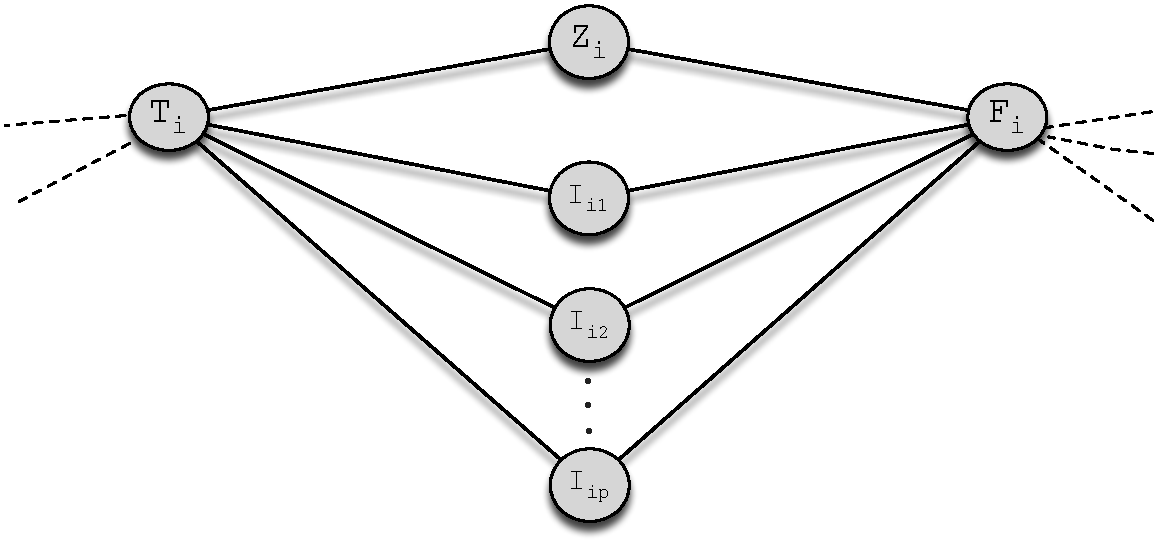
\includegraphics[scale=0.41]{figs/extensions/vgadget-inject-extend.pdf}}
    \subfigure[Modified variable gadget used in \xval and \xvalparts. Each disconnected subgraph has additional injection nodes: nodes $I_{i1}^t, I_{i2}^t, \dots I_{ip}^t$ are added to the upper subgraph
	and nodes $I_{i1}^b, I_{i2}^b, \dots I_{ip}^b$ are included in the bottom subgraph.]
	 {\label{fig:variable-inject-extend2}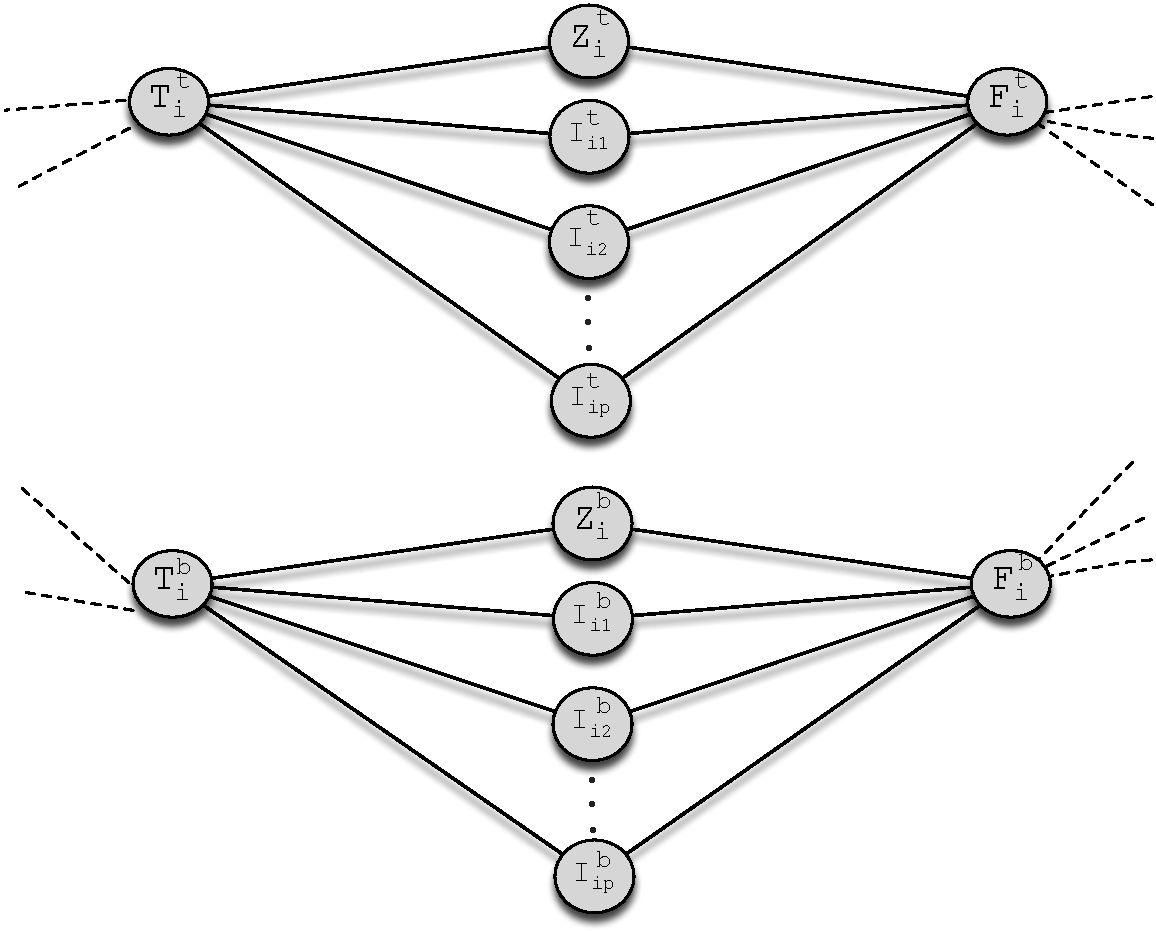
\includegraphics[scale=0.41]{figs/extensions/vgadget-inject-extend2.pdf}}
  \end{center}
	\caption{Figures for variable gadget extensions to include more injection nodes described in Section \ref{subsec:extend}. The dashed edges indicate connections to clause gadget nodes. }
\end{figure}

\begin{figure}[t]
  \begin{center}
    \subfigure[Modified variable gadget used in \full and \maxincs, containing additional injection nodes: $Z_{i1}, Z_{i2}, \dots Z_{ip}$. ]{\label{fig:variable-noninject-extend}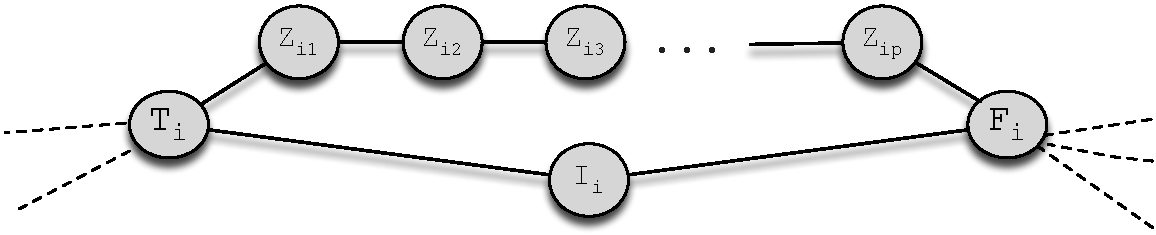
\includegraphics[scale=0.41]{figs/extensions/vgadget-noninject-extend.pdf}}
    \subfigure[Modified variable gadget used in \xval and \xvalparts. Each disconnected subgraph has additional injection nodes: the upper subgraph includes nodes $Z_{i1}^t, Z_{i2}^t, \dots Z_{ip}^t$
	 and nodes  $Z_{i1}^b, Z_{i2}^b, \dots Z_{ip}^b$ are added in the bottom subgraph.]
	 {\label{fig:variable-noninject-extend2}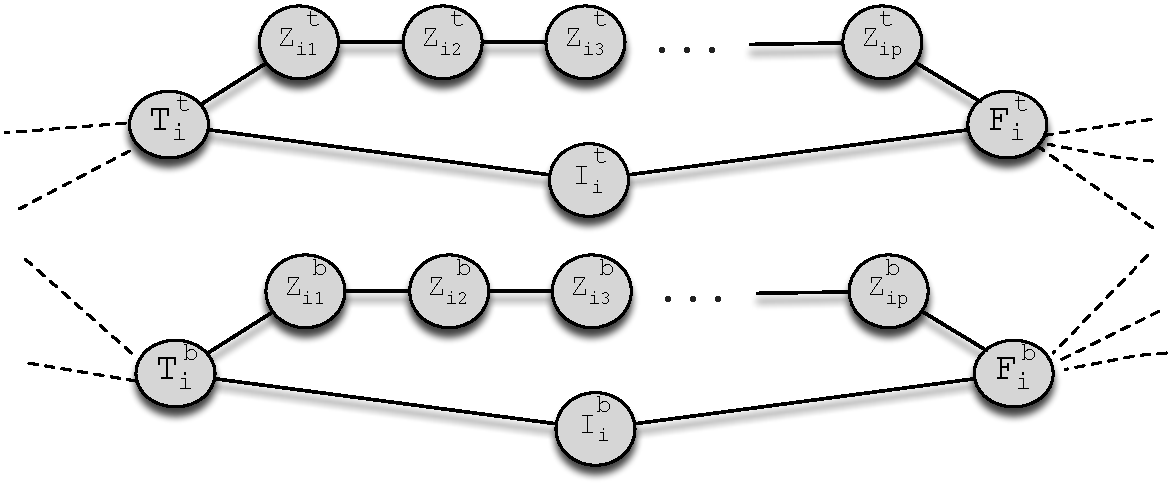
\includegraphics[scale=0.41]{figs/extensions/vgadget-noninject-extend2.pdf}}
  \end{center}
	\caption{Figures for variable gadget extensions to include more non-injection nodes described in Section \ref{subsec:extend}. The dashed edges indicate connections to clause gadget nodes. }
\end{figure}



\begin{figure}[t]
\centering
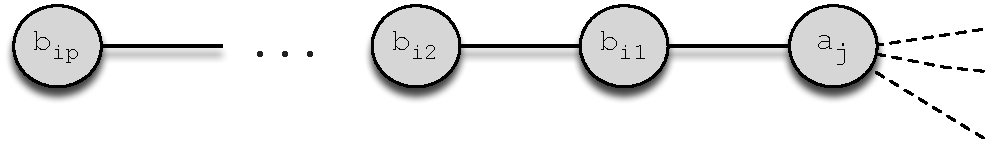
\includegraphics[scale=0.49]{figs/extensions/line-gadget-extend.pdf}
%\includegraphics[scale=0.51]{figs/example2.pdf}
\caption{Extended clause gadget, $C_j'$, used in Section \ref{subsec:extend}. All nodes are injection nodes.}
\label{fig:clause-extend}
\end{figure}




\section{Approximation Algorithms}
\label{sec:approx}

Because all four placement problems are NPC, we propose greedy approximation algorithms for each problem, which iteratively add 
a PMU in each step to the node that observes the maximum number of new nodes. We present two such algorithms, one which directly addresses \maxinc ({\tt greedy}) and the other 
\xvalpart ({\tt xvgreedy}). {\tt greedy} and {\tt xvgreedy} can easily be used to solve \full and \xvals, respectively, by selecting the appropriate $k$ value to ensure full observability.
We prove these algorithms have polynomial complexity (i.e., they are in $\mathcal{P}$), making them feasible tools for approximating optimal PMU placement. 

{\bf {\tt greedy} Algorithm}. We start with $\Phi = \emptyset$.  At each iteration, we add a PMU to the node that results in the observation of the maximum number of 
new nodes. The algorithm terminates when all PMUs are placed.  {\footnote {\small This is the same greedy algorithm proposed by Aazami and Stilp \cite{Aazami07}. }}
The pseudo-code for {\tt greedy} is given in Algorithm \ref{alg:greedy}.
%We refer to this algorithm as {\tt greedy} and give the pseudo-code in Algorithm \ref{alg:greedy}.

\begin{algorithm}
\caption{{\tt greedy} with input $G=(V,E)$ and $k$ PMUs}
\label{alg:greedy}

\begin{algorithmic}[1]

\STATE{$\Phi_G \leftarrow \emptyset$}
\FOR{$k$ iterations}
	\STATE{$maxObserved \leftarrow 0$}
	\FOR{{\bf each} $v \in (V - \Phi_G$)}
		\STATE{$numObserved \leftarrow 0$}
		\FOR{{\bf each} $u \in (\Phi_G \cup \{v\})$}
			\STATE{add PMU to $u$}
			\STATE{apply O1 at $u$ and update $numObserved$}
		\ENDFOR
		\REPEAT
			\STATE{$flag \leftarrow False$}
			\FOR{{\bf each} $w \in (V - (\Phi_G \cup \{v\}))$}
				\IF{$w \in (V_Z \cap \Phi_G^R)$ and $w$ has $1$ unobserved neighbor}
					\STATE{apply O2 at $w$ and update $numObserved$}
					\STATE{$flag \leftarrow True$}
				\ENDIF
			\ENDFOR
		\UNTIL{$flag = False$}
		\IF{$numObserved > maxObserved$}
			\STATE{$greedyNode \leftarrow v$}
			\STATE{$maxObserved \leftarrow numObserved$}
		\ENDIF
	\ENDFOR
	\STATE{$\Phi_G \leftarrow \Phi_G \cup \{greedyNode\}$}
\ENDFOR
\end{algorithmic}
\end{algorithm}

\begin{theorem}
For input graph $G=(V,E)$ and $k$ PMUs {\tt greedy} has $O(dkn^3)$ complexity, where $n=|V|$ and $d$ is the maximum degree node in $V$.
\label{thm:greedy-complex}
\end{theorem}
\begin{proof}
%In our proof we implicitly refer to Algorithm \ref{alg:greedy} when referring to the steps of the algorithm.
%Specifically, when we refer to the {\tt greedy} algorithm steps we are referencing the Algorithm \ref{alg:greedy} steps.
The procedure to determine the number of nodes observed by a candidate PMU placement spans steps $6 - 18$.
{\footnote {\small In this proof, step $i$ refers to the $i^{th}$ line  in Algorithm \ref{alg:greedy}.}}
First, we apply O1 at each PMU node (steps $6 -9$). O1 takes $O(d)$ time 
to be applied at a single node.  Because $|\Phi_G| \leq k$, the total time to apply O1 is $O(dk)$. 

Then, we iteratively apply O2 (steps $10-18$), terminating when no new nodes are observed.  Like O1, applying O2 at a single node takes $O(d)$ time. 
In each iteration, if possible we apply O2 at each $v \in (V_Z \cap \Phi_G^R)$ (steps $13-16$). %If at least one node is observed we execute another iteration of O2 evaluation.
It total, the $loop$ spanning steps $10-18$ repeats at most $O(n)$ times.  This occurs when only a single new node is observed in each iteration.  The $for$ loop spanning steps $12-17$
repeats $O(n)$ times. We conclude that O2 evaluation for each set of candidate PMU locations takes $O(dn^2)$ time.

In order to determine the placement of each PMU, we try all possible PMU placements among nodes without a PMU. We place the PMU at the node that observes the maximum number of new nodes.  This 
corresponds to Steps $4-23$, in which the $for$ loop iterates $O(n)$ times. 
Thus the complexity of Steps $4-23$ is $O(dn^3)$. 

Finally, the outer most $for$ loop (Steps $2-25$) iterates $k$ times: one iteration
to determine the greedy placement of each PMU.  We conclude that the complexity of {\tt greedy} is $O(dkn^3)$. \qed
\end{proof}
%At most, O2 evaluation requires $O(n)$ iterations in which we attempt to apply O2 at $O(n)$ nodes. This yields $O(n^2)$ complexity.



%After placing PMUs in candidate locations, we apply rule O1 at each PMU node.  It takes $O(d)$ time, where $d$ is the maximum degree of all $v \in V$, to apply O1 at each PMU node.  With 
%$k$ PMUs, the total time to apply O1 is $O(kd)$.


{\bf {\tt xvgreedy} Algorithm}. {\tt xvgreedy} is almost identical to {\tt greedy}, except that PMUs are added in pairs such that the selected pair observe
the maximum number of nodes under the condition that the PMU pair satisfy one of the cross-validation rules. % and observe the maximum number of new nodes.
We provide the pseudo code for {\tt xvgreedy} in Algorithm \ref{alg:xvgreedy}.
%We call this algorithm {\tt xvgreedy} and provide pseudo code for {\tt xvgreedy} in Algorithm \ref{alg:xvgreedy}.

\begin{algorithm}
\caption{{\tt xvgreedy} with input $G=(V,E)$ and $k$ PMUs}
\label{alg:xvgreedy}

\begin{algorithmic}[1]

\STATE{$\Phi_G \leftarrow \emptyset$}
\FOR{$k$ iterations}
	\STATE{$maxObserved \leftarrow 0$}
	\STATE{$C \leftarrow$ all cross-validated node pairs in $(V - \Phi_G)$}
	\FOR{{\bf each} $\{v_1,v_2\} \in C$}
		\STATE{$numObserved \leftarrow 0$}
		\FOR{{\bf each} $u \in (\Phi_G \cup \{v_1,v_2\})$}
			\STATE{add PMU to $v_1$ and $v_2$}
			\STATE{apply O1 at $u$ and update $numObserved$}
		\ENDFOR
		\REPEAT
			\STATE{$flag \leftarrow False$}
			\FOR{{\bf each} $w \in (V - (\Phi_G \cup \{v_1,v_2\}))$}
				\IF{$w \in (V_Z \cap \Phi_G^R)$ and $w$ has $1$ unobserved neighbor}
					\STATE{apply O2 at $w$ and update $numObserved$}
					\STATE{$flag \leftarrow True$}
				\ENDIF
			\ENDFOR
		\UNTIL{$flag = False$}
		\IF{$numObserved > maxObserved$}
			\STATE{$greedyNodes \leftarrow \{v_1,v_2\}$}
			\STATE{$maxObserved \leftarrow numObserved$}
		\ENDIF
	\ENDFOR
	\STATE{$\Phi_G \leftarrow \Phi_G \cup greedyNodes$}
\ENDFOR
\end{algorithmic}
\end{algorithm}

\begin{theorem}
For input graph $G=(V,E)$ and $k$ PMUs {\tt xvgreedy} has $O(kdn^3)$ complexity, where $n=|V|$ and $d$ is the maximum degree node in $V$.
\label{thm:xvgreedy-complex}
\end{theorem}
\begin{proof}
	The only difference between {\tt xvgreedy} and {\tt greedy} is that {\tt xvgreedy} only considers pairs of cross-validated nodes. For this reason, 
	step $4$ in Algorithm \ref{alg:xvgreedy} does not appear in Algorithm \ref{alg:greedy}.  We can find all pairs of cross-validated nodes in $O(d^2n)$ time.  We do so by 
	implementing a breadth-first search at each $v \in (V - \Phi_G)$ but stopping at a depth of $2$.  This takes $O(d^2)$ time for each node and since 
	$O(n)$ searches are executed, step $4$ takes $O(d^2n)$ time.

	Because all other parts of Algorithm \ref{alg:greedy} and Algorithm \ref{alg:xvgreedy} are nearly identical -- Algorithm \ref{alg:xvgreedy}
	adds PMUs in pairs while Algorithm \ref{alg:greedy} adds PMUs one-at-a-time -- we are able to directly apply
	the analysis from Theorem \ref{thm:greedy-complex} in this proof.  Therefore, we conclude the complexity of {\tt xvgreedy} is $O(k(d^2n + dn^3)) = O(dkn^3)$. \qed
\end{proof}







%\xvals's greedy algorithm can either:
%\begin{itemize}
%	\item Add pairs of PMUs at each iteration such the selected pair of nodes observes the most nodes. both nodes need to be unobserved. pros/cons
%	\begin{itemize}
%		\item ignores odd number of PMUs
%	\end{itemize}
%	\item Add a single PMU at each iteration so the PMU is cross-validated and observes the maximum nodes (among the cross-validated options). pros/cons
%	\begin{itemize}
%		\item may be better to add PMUs in pairs
%
%		\item may restrict options by having to place nodes near each other ...
%	\end{itemize}
%
%\end{itemize}

 

% DON'T USE THE TECH VERSION, OUTDATED (7/24/12)
\section{Simulation Study}
\label{sec:simulations}

\textbf{Topologies.} 
We evaluate our approximation algorithms with simulations over synthetic topologies generated using real portions of the North American electric power grid 
(i.e., IEEE bus systems $14$, $30$, $57$, and $118$) as templates \footnote{\url{http://www.ee.washington.edu/research/pstca/}}. 
The bus system number indicates the number of nodes in the graph (e.g., bus system $57$ has $57$ nodes).
It is standard practice in the literature to only use single IEEE bus systems \cite{Baldwin93,Abur06,Mili90,Xu04}.  
We follow this precedent but do not present these results because they are consistent with the trends found using synthetic topologies.
Instead, we focus on synthetic topologies because, unlike simulations using single IEEE bus systems, we can establish the statistical significance of the performance of our greedy approximations.

Since observability is determined by the connectivity of the graph, we use the {\em degree distribution} of IEEE topologies as the template for generating our synthetic graphs.
A synthetic topology is generated from a given IEEE graph by randomly ``swapping'' edges in the IEEE graph. Specifically, we select a random $v \in V$ and then pick a random $u \in \Gamma(v)$. 
Let $u$ have degree $d_u$.  Next, we select a random $w \notin \Gamma(v)$ with degree $d_w = d_u -1$. % {\footnote {\small Here ``random'' means uniformly at random.}
Finally, we remove edge $(v,u)$ and add $(v,w)$, thereby preserving the node degree distribution.
We continue this swapping procedure until the original graph and generated graph share {\em no edges}, and then return the resulting graph.

\textbf{Evaluation Methods.}
We are interested in evaluating how close our algorithms are to the optimal PMU placement. 
Thus, when computationally possible (for a given $k$) we use brute-force algorithms to iterate over all possible placements of $k$ PMUs in a given graph and select the best PMU placement. 
When the brute-force algorithm is computationally infeasible, we present only the performance of the greedy algorithm.
In what follows, the output of the brute-force algorithm is denoted {\tt optimal}, and when we require cross-validation it is denoted {\tt xvoptimal}.

%We consider performance as a function of the number of PMUs,
%We present three different simulations in Section \ref{subsec:synth}-\ref{subsec:ieee}. 
%In Section \ref{subsec:synth} we consider performance as a function of the number of PMUs, and
%in Section \ref{subsec:zero} we investigate the performance impact of the number of zero-injection nodes in the network.
%These two sections use synthetic graphs. We conclude in Section \ref{subsec:ieee}, where we compare these results to the performance over the actual IEEE graphs.

%\subsection{Simulation 1: Impact of Number of PMUs}
%\label{subsec:synth}

\textbf{Simulation Results.}
We vary the number of PMUs and determine the number of observed nodes in the synthetic graph. 
Each data point is generated as follows. For a given number of PMUs, $k$, we generate a graph, place $k$ PMUs on the graph, and then determine the number of observed nodes. 
We continue this procedure until $[0.9(\overline{x}),1.1(\overline{x})]$ -- where $\overline{x}$ is the mean number of observed nodes using $k$ PMUs -- falls within the $90\%$ confidence interval.

In addition to generating a topology, for each synthetic graph we determined the members of $V_I, V_Z$. These nodes are specified for the original graphs in the IEEE bus system database. Thus, 
we randomly map each node in the IEEE graph to a node in the synthetic graph with the same degree, and then match their membership to either $V_I$ or $V_Z$.

%We present here results for solving \maxinc and \xvalpart using synthetic graphs based on IEEE bus $57$.  
Due to space constraints, we only show plots for solving \maxinc and \xvalpart using synthetic graphs based on IEEE bus $57$.  
The number of nodes observed given $k$, using {\tt greedy} and {\tt optimal}, are shown in Figure \ref{fig:bus57}, and Figure \ref{fig:xvbus57} shows this number 
for {\tt xvgreedy} and {\tt xvoptimal}.  Both plots include the $90\%$ confidence intervals. 
Results for synthetic graphs generated using IEEE bus $14$, $30$, and $118$ yield the same trends.

Our greedy algorithms perform well. On average, {\tt greedy} is within $98.6\%$ of {\tt optimal},
is never below $94\%$ of {\tt optimal}, and in most cases gives the optimal result.
Likewise, {\tt xvgreedy} is never less than $94 \%$ of {\tt xvoptimal} and on average is within $97\%$ of {\tt xvoptimal}. In about about half the cases {\tt xvgreedy} gives the optimal result.
These results suggest that despite the complexity of the problems, a greedy approach can return high-quality results. Note, however, that these statistics do not include performance when
$k$ is large.  It is an open question whether {\tt greedy} and {\tt xvgreedy} would do well for large $k$. 

Surprisingly, when comparing our results with and without the cross-validation requirement, we find that the cross-validation constraints have little effect on the number of observed nodes 
for the same $k$. Our experiments show that on average {\tt xvoptimal} observed only $5\%$ fewer nodes than {\tt optimal}.  Similarly, on average {\tt xvgreedy} observes
 $5.7\%$ fewer nodes than {\tt greedy}. This suggests that the cost of imposing the cross-validation requirement is low, with the clear gain of ensuring PMU correctness across the network.


\begin{figure*}[t]
  \begin{center}
    \subfigure[{\tt greedy} vs {\tt optimal}]{\label{fig:bus57}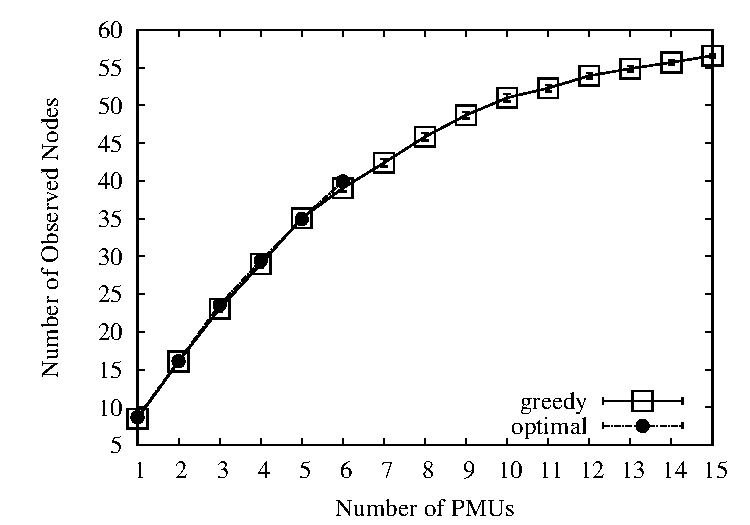
\includegraphics[scale=0.59]{figs/bus57.pdf}}
    \subfigure[{\tt xvgreedy} vs {\tt xvoptimal}]{\label{fig:xvbus57}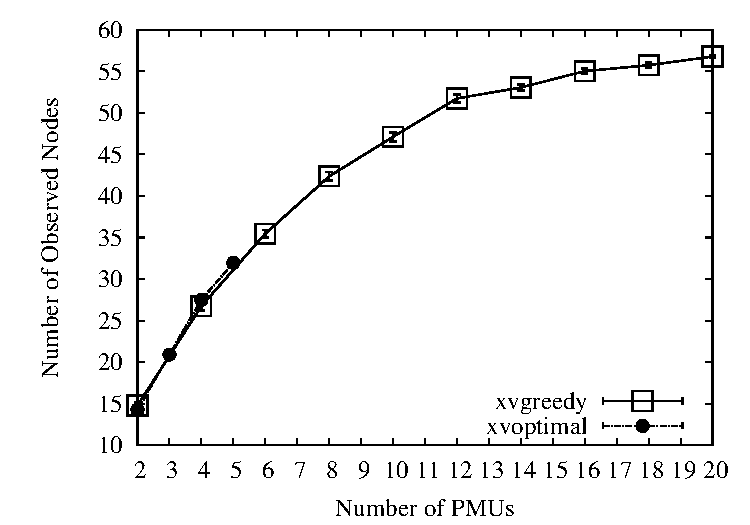
\includegraphics[scale=0.59]{figs/xvbus57.pdf}}
  \end{center}
	\caption{Mean number of observed nodes over synthetic graphs based on IEEE bus $57$ when varying number of PMUs. The $90\%$ confidence interval is shown.}
\end{figure*}







%\section{Simulations}
\label{sec:simulations}

\textbf{Topologies.} We evaluate our approximation algorithms using simulations over IEEE topologies as well as synthetic ones. For IEEE topologies, we use bus systems $14$, $30$, $57$, and $118$
{\footnote {\small http://www.ee.washington.edu/research/pstca/}}.  The bus system number indicates the number of nodes in the graph (e.g., bus system $57$ has $57$ nodes).
Synthetic graphs are then generated based on each of these topologies, and are used to quantify the performance of our greedy approximations.
%For each algorithm, we determine the number of nodes that are observed by placing $k$ PMUs on IEEE bus systems $14$, $30$, $57$, and $118$.
%{\footnote {\small http://www.ee.washington.edu/research/pstca/}} as well as synthetic graphs generated by using these IEEE graphs as templates.

Since observability is determined by the connectivity of the graph, we use the {\em degree distribution} of IEEE topologies as the template for generating our synthetic graphs.
%In Section \ref{subsec:ieee}, we compare the results we get for the synthetic graphs with those of the IEEE topologies.
A synthetic topology is generated from a given IEEE graph by randomly ``swapping'' edges in the IEEE graph. Specifically, we select a random $v \in V$ and then pick a random $u \in \Gamma(v)$. 
Let $u$ have degree $d_u$.  Next, we select a random $w \notin \Gamma(v)$ with degree $d_w = d_u -1$.  {\footnote {\small Here ``random'' means uniformly at random.}
Finally, we remove edge $(v,u)$ and add $(v,w)$, thereby preserving the node degree distribution.
We continue this swapping procedure until the original graph and generated graph share {\em no edges}, and then return the resulting graph.
%Note that this edge-swapping procedure ensures that the degree distribution of each generated graph is identical to the degree distribution of the original bus system.

\textbf{Evaluation Methods.}
We are interested in evaluating how close our algorithms are to the optimal PMU placement. 
%Ideally, we would like to compare the performance of our greedy algorithms with the optimal PMU placement.
Thus, when computationally possible (for a given $k$) we use brute-force algorithms to iterate over all possible placements of $k$ PMUs in a given graph and select the best PMU placement. When computationally infeasible, we present only the performance of the greedy algorithm without corresponding optimal solutions.
In what follows, the output of the brute-force algorithm is denoted {\tt optimal}, and when we require cross-validation it is denoted {\tt xvoptimal}.
%For \xval and \xvalparts, we do the same while ignoring PMU placements that do not meet cross-validation requirements. We use {\tt xvoptimal} to refer to this algorithm.
%For \xval and \xvalparts, we ignore PMU placements which do not meet the cross-validation rules described in Section \ref{subsec:xval}.

%For large graphs, the exponential runtime of this brute force algorithm makes computation infeasible. Thus, we have no optimal results for IEEE bus systems $57,118$ for large $k$  and their corresponding synthetic graphs. For this reason, the {\tt optimal} and {\tt xvoptimal} curves stop abruptly in the corresponding plots. %Figure \ref{fig:bus57}|, \ref{fig:bus118}, Figure \ref{fig:xvbus118}, and Figure \ref{fig:all118}.

We present three different simulations in Section \ref{subsec:synth}-\ref{subsec:ieee}. 
%In Sections \ref{subsec:synth}-\ref{subsec:ieee} we investigate the performance of our algorithms as well as the network PMU requirements.  
In Section \ref{subsec:synth} we consider performance as a function of the number of PMUs, and in Section \ref{subsec:zero} we investigate the performance impact of the number of zero-injection nodes in the network. These two sections are performed over sets of synthetic graphs. We conclude in Section \ref{subsec:ieee} where we compare these results to the performance over the actual IEEE graphs.

\subsection{Simulation 1: Impact of Number of PMUs}
\label{subsec:synth}

In the first simulation scenario we vary the number of PMUs and determine the number of observed nodes in the synthetic graph.  %We do so for both with and without cross-validation.
Each data point is generated as follows. For a given number of PMUs, $k$, we generate a graph, place $k$ PMUs on the graph, and then determine the number of observed nodes. 
We continue this procedure until $[0.9(\overline{x}),1.1(\overline{x})]$ -- where $\overline{x}$ is the mean number of observed nodes using $k$ PMUs -- falls within the $90\%$ confidence interval.

In addition to generating a topology, for each synthetic graph we determined the members of $V_I, V_Z$. These nodes are specified for the original graphs in the IEEE bus system database. Thus, 
we randomly map each node in the IEEE network to a node in the synthetic network with the same degree, and then match their membership to either $V_I$ or $V_Z$.

We present here results for solving \maxinc and \xvalparts.  The number of nodes observed given $k$, using {\tt greedy} and {\tt optimal}, are shown in Figure \ref{fig:maxinc-res}, and Figure \ref{fig:xv-res} shows this number for {\tt xvgreedy} and {\tt xvoptimal}. In both sets of plots we show $90\%$
confidence intervals. We omit results for graphs based on IEEE bus $14$ because the same trends are observed.

Our greedy algorithms perform well. On average, {\tt greedy} is within $98.6\%$ of {\tt optimal},
is never below $94\%$ of {\tt optimal}, and in most cases gives the optimal result.
Likewise, {\tt xvgreedy} is never less than $94 \%$ of {\tt xvoptimal} and on average is within $97\%$ of {\tt xvoptimal}. In about about half the cases {\tt xvgreedy} gives the optimal result.
These results suggest that despite the complexity of the problems, a greedy approach can return high-quality results. Note, however, that these statistics do not include performance over
large topologies (i.e., IEEE graphs $57, 118$) when $k$ is large.  It is an open question whether the greedy algorithms used here would do well for larger graphs.
%Typically, greedy algorithms fail because they commit to a choice too early
%and do not reconsider earlier decisions.  Our results suggest that this is not the case for our PMU placement problems.

%However, these statistics do not include a comparison of greedy versus optimal for large $k$ values in the graphs generated from IEEE graphs $57$ and $118$.
%This is the case because the exponential running time of {\tt optimal} and {\tt xvoptimal} for these inputs made computing a result infeasible.
%Therefore, it is unknown if {\tt greedy} and {\tt xvgreedy} yields results as close to optimal for these inputs.

Surprisingly, when we compare our results with and without the cross-validation requirement, we find that this set of constraints does not have a significant effect on the number of observed nodes for the same $k$. Our experiments show that on average {\tt xvoptimal} observed only $5\%$ fewer nodes than {\tt optimal}.  Similarly, on average {\tt xvgreedy} observes
 $5.7\%$ fewer nodes than {\tt greedy}. This suggests that the cost of imposing this requirement is low, with the clear gain of ensuring PMU correctness across the network via cross-validation. 

%when compared to our greedy solution for the corresponding buses. 

%\begin{figure*}[t]
%  \begin{center}
%    \subfigure[Graphs based on IEEE Bus $30$]{\label{fig:bus30}\includegraphics[scale=0.45]{figs/allbus30.pdf}}
%    \subfigure[Graphs based on IEEE Bus $57$]{\label{fig:bus57}\includegraphics[scale=0.45]{figs/allbus57.pdf}}
%    \subfigure[Graphs based on IEEE Bus $118$]{\label{fig:bus118}\includegraphics[scale=0.45]{figs/allbus118.pdf}}
%  \end{center}
%	\caption{Mean number of observed nodes over synthetic graphs -- using {\tt greedy}, {\tt xvgreedy}, {\tt optimal}, and {\tt xvoptimal} -- 
%	when varying number of PMUs. The $90\%$ confidence interval is shown.}
%  \label{fig:maxinc-res}
%\end{figure*}

\begin{figure*}[t]
  \begin{center}
    \subfigure[Graphs based on IEEE Bus $30$]{\label{fig:bus30}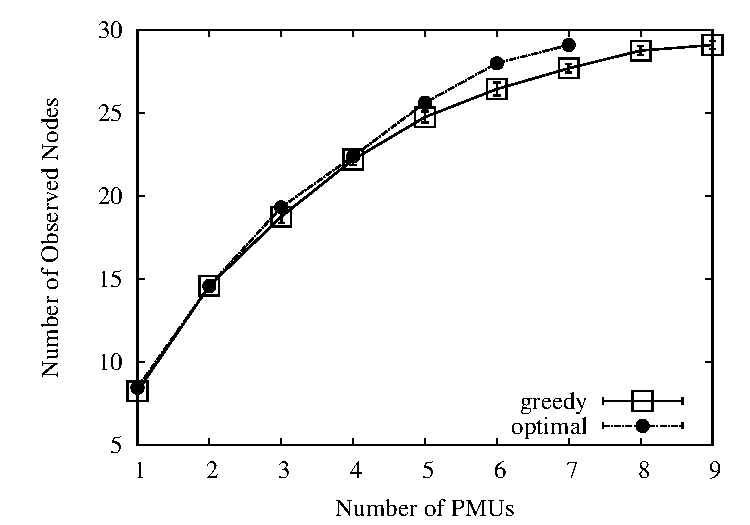
\includegraphics[scale=0.45]{figs/bus30.pdf}}
    \subfigure[Graphs based on IEEE Bus $57$]{\label{fig:bus57}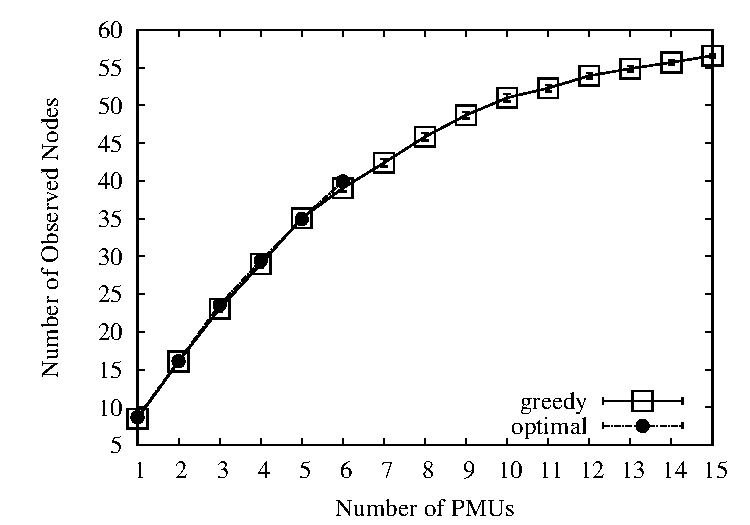
\includegraphics[scale=0.45]{figs/bus57.pdf}}
    \subfigure[Graphs based on IEEE Bus $118$]{\label{fig:bus118}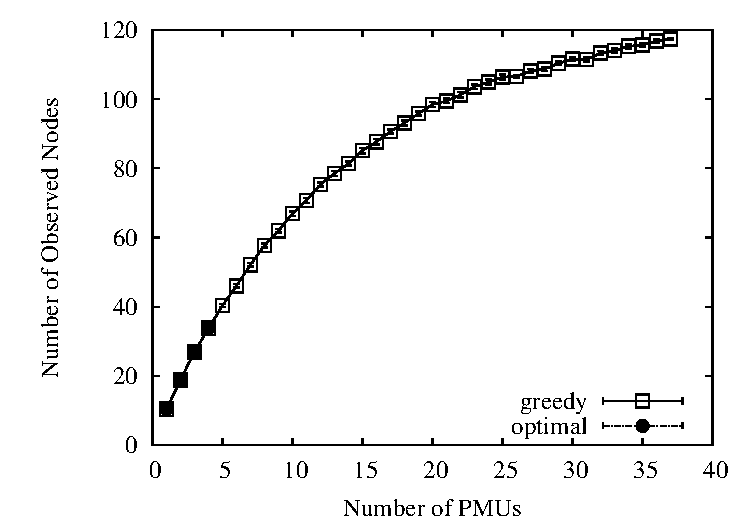
\includegraphics[scale=0.45]{figs/bus118.pdf}}
  \end{center}
	\caption{Mean number of observed nodes over synthetic graphs -- using {\tt greedy} and {\tt optimal} -- when varying number of PMUs. The $90\%$ confidence interval is shown.}
  \label{fig:maxinc-res}
\end{figure*}

\begin{figure*}[t]
  \begin{center}
    \subfigure[Graphs based on IEEE Bus $30$]{\label{fig:xvbus30}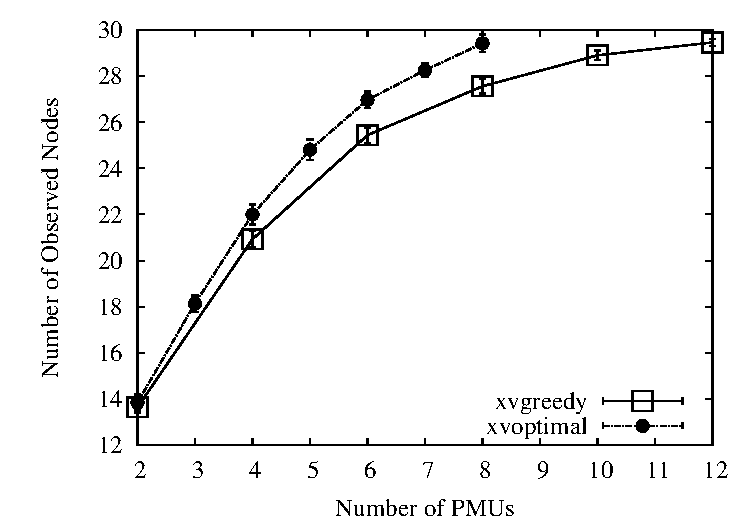
\includegraphics[scale=0.45]{figs/xvbus30.pdf}}
    \subfigure[Graphs based on IEEE Bus $57$]{\label{fig:xvbus57}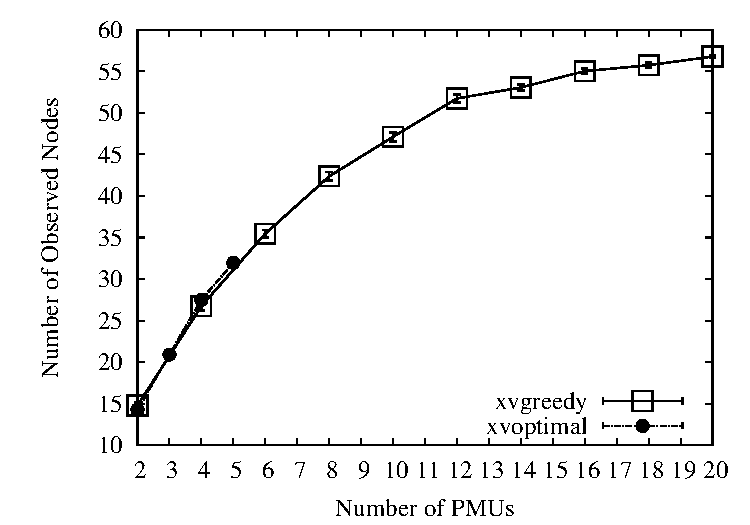
\includegraphics[scale=0.45]{figs/xvbus57.pdf}}
    \subfigure[Graphs based on IEEE Bus $118$]{\label{fig:xvbus118}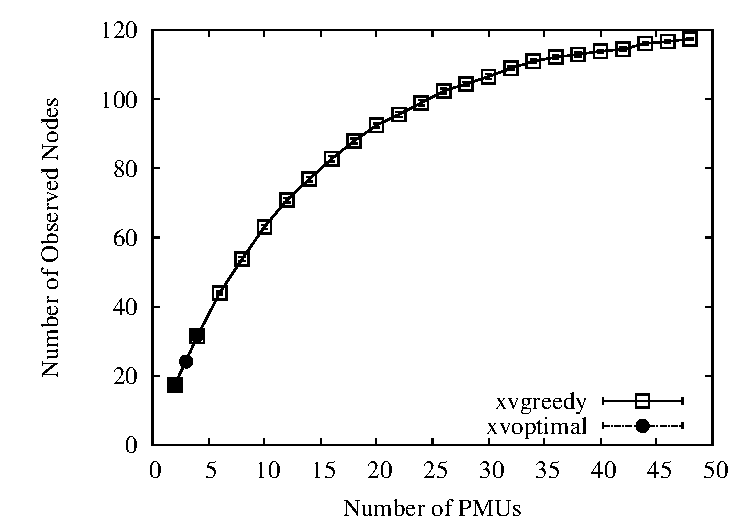
\includegraphics[scale=0.45]{figs/xvbus118.pdf}}
  \end{center}
	\caption{Over synthetic graphs, mean number of observed nodes -- using {\tt xvgreedy} and {\tt xvoptimal} -- when varying number of PMUs. The $90\%$ confidence interval is shown.}
  \label{fig:xv-res}
\end{figure*}




%\begin{figure}[t]
%\centering
%\includegraphics[scale=0.50]{figs/all118.pdf}
%\caption{Simulation results for \maxinc and \xvalpart using IEEE bus $118$.}
%\label{fig:all118}
%\end{figure}

\subsection{Simulation 2: Impact of Number of Zero-Injection Nodes}
\label{subsec:zero}

Next, we examine the impact of $|V_Z|$ on algorithm performance. 
For each synthetic graph, we run our algorithms for increasing values of $|V_Z|$ and determine the minumum number of PMUs needed to observe all nodes in the graph ($k^*$).
For each $z:=|V_Z|$, we select $z$ nodes uniformly at random to be zero-injection, and the rest are in $V_I$. Because we compute $k^*$ here, we solve \full and \xvals, rather than
\maxinc and \xvalparts as in Simulation 1.

We generate each data point using a similar procedure to the one described in Section \ref{subsec:synth}.  
For each $z=z_i$, we generate a graph and determine $k^*$. %the minimum number of PMUs needed to observe all nodes in the graph ($k^*$).  
We then compute $\overline{k^*}$, the mean value of $k^*$ over all simulation runs with $|V_Z| = z_i$.
We continue this procedure until $[0.9(\overline{k^*}),1.1(\overline{k^*})]$ falls within the $90\%$ confidence interval.

Figure \ref{fig:zero57} shows the simulation results for solving \full and \xval on synthetic graphs modeled by IEEE bus $57$. Results for other topologies considered here 
(i.e., $14$, $30$ and $118$) followed the same trend and are thus omitted. Due to the exponential running time of {\tt optimal} and {\tt xvoptimal}, we present here only results of our 
greedy algorithms. 

As expected, increasing the number of zero-injection nodes -- for both {\tt greedy} and {\tt xvgreedy} -- reduces the number of PMUs required for 
full observability. 
More zero-injection nodes allow O2 to be applied more frequently (Figure \ref{fig:o2}), thereby increasing the number of observed nodes without using more PMUs.
In fact, we found the relationship between $|V_Z|$ to the greedy estimate of $k^*$  to be linear.

The gap in $k^*$ between {\tt greedy} and {\tt xvgreedy} decreases as $z$ grows. {\tt greedy} and {\tt xvgreedy} observe a similar
number of nodes via O2 across all $z$ values: the mean absolute difference in the number of nodes observed by O2 between the two algorithms is $1.66$ nodes.  
Thus, as $z$ grows the number of nodes observed by O2 accounts for an increasing proportion of all observed nodes (Figure \ref{fig:o2}), causing the gap between {\tt greedy} and {\tt xvgreedy} to shrink.
%This statistic is confirmed visually by referring to Figure \ref{fig:o2} where the error bars (e.g., the $90\%$ confidence interval) for each data point are overlapping.  Thus, the number of nodes observed by O1 
%-- {\tt greedy} observes more nodes via O1 than {\tt xvgreedy} -- accounts for the difference between the two greedy algorithms. 
%We conclude that becuase the number of O2 observed nodes increases super-linearly with $z$ the gap between {\tt greedy} and {\tt xvgreedy} shrinks.


%\begin{figure*}[t]
%  \begin{center}
%    \subfigure[Graphs based on IEEE Bus $30$]{\label{fig:xvbus30}\includegraphics[scale=0.45]{figs/zero30.pdf}}
%    \subfigure[Graphs based on IEEE Bus $57$]{\label{fig:xvbus57}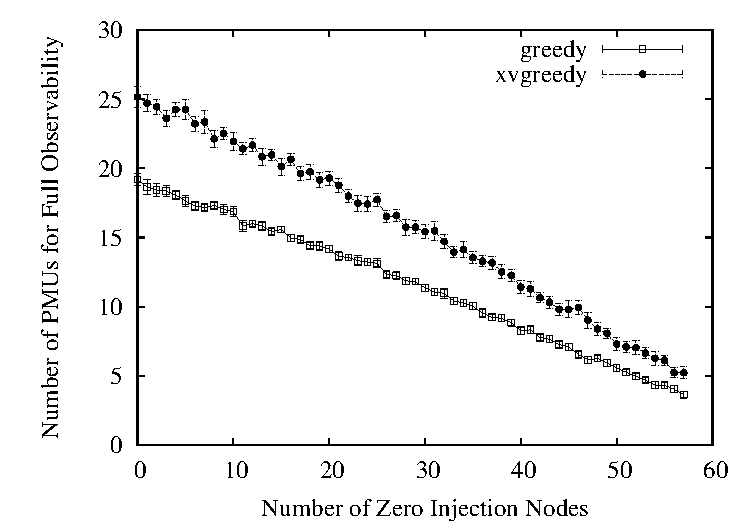
\includegraphics[scale=0.45]{figs/zero57.pdf}}
%    \subfigure[Graphs based on IEEE Bus $118$]{\label{fig:xvbus118}\includegraphics[scale=0.45]{figs/zero118.pdf}}
%  \end{center}
%	\caption{Simulation Results for \full and \xval greedy approximations, in which we vary the number of zero-injection nodes and determine the minimum number of PMUs needed to observe all nodes. 
%	{\tt xvgreedy} refers to the greedy algorithm with cross-validation and {\tt greedy} denotes the greedy algorithm without cross-validation. The $90\%$ confidence interval is shown. }
%  \label{fig:zero}
%\end{figure*}

\begin{figure*}[t]
  \begin{center}
    \subfigure[\un{Simulation 2}: Number of PMUs needed for full observability for different $|V_Z|$ values, using synthetic graphs based on IEEE Bus $57$.]{\label{fig:zero57}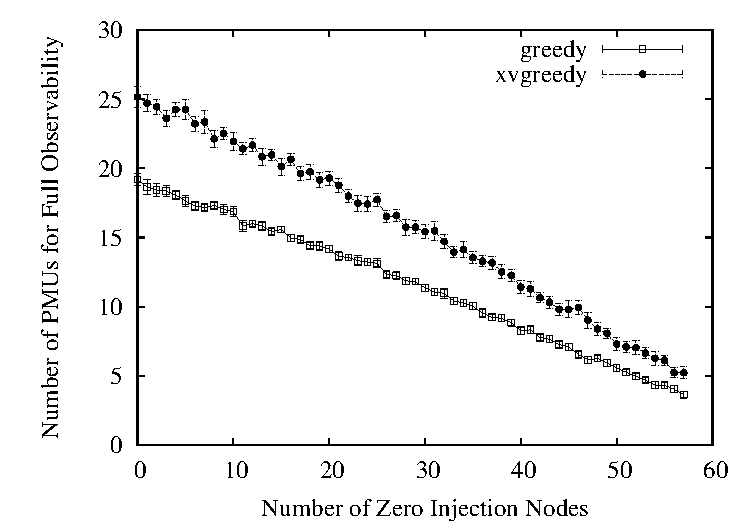
\includegraphics[scale=0.45]{figs/zero57.pdf}}
    \subfigure[\un{Simulation 2}: Number of nodes observed by O2 for different $|V_Z|$ values, using synthetic graphs based on IEEE Bus $57$.] {\label{fig:o2}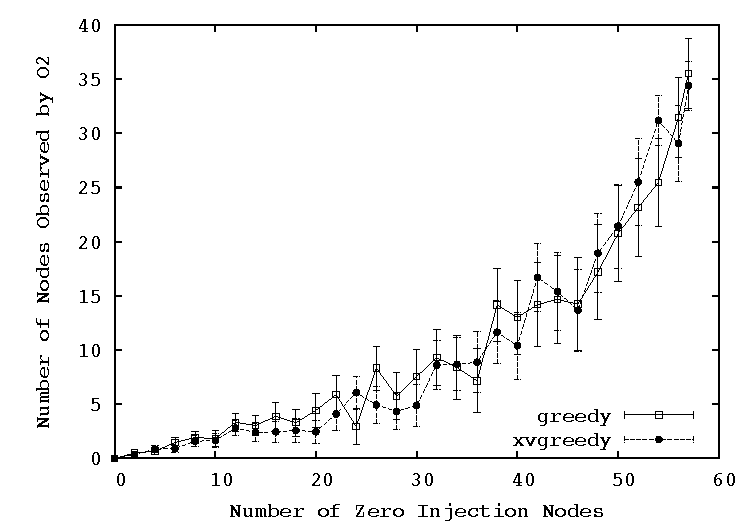
\includegraphics[scale=0.45]{figs/o2-b57.pdf}}
    \subfigure[\un{Simulation 3}: Number of observed nodes when varying number of PMUS, using IEEE Bus $57$]{\label{fig:single57}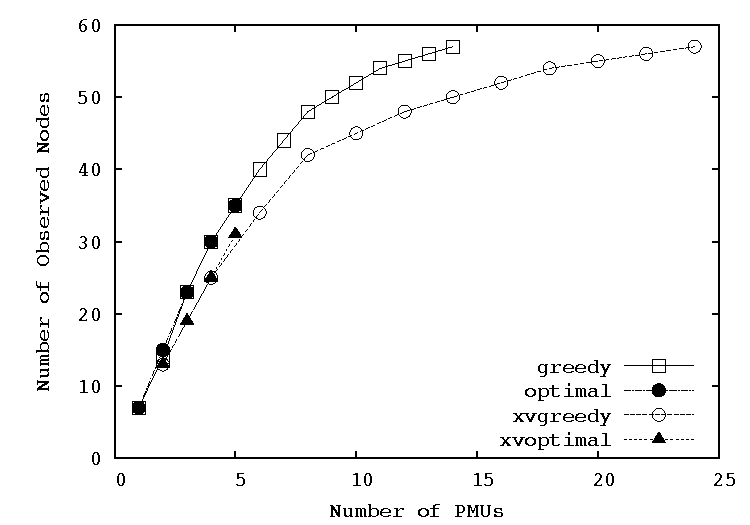
\includegraphics[scale=0.45]{figs/bus-single57.pdf}}
  \end{center}
	\caption{Results for Simulation 2 and 3. In Figures (a) and (b) the $90\%$ confidence interval is shown. }
  \label{fig:sim23}
\end{figure*}


\subsection{Simulation 3: Synthetic vs Actual IEEE Graphs}
\label{subsec:ieee}
In this section, we compare our results with the performance over the original IEEE systems. 
We assign nodes to $V_Z$ and $V_I$ as specified in the IEEE database files. Our results indicate that the trends we observed over the synthetic graphs apply as well to real topologies.


%When repeating Simulation 1, we find the same trends using the IEEE topologies. %as with the synthetic graphs.
Figure \ref{fig:single57} shows the number of observed nodes for the {\tt greedy},  {\tt xvgreedy}, {\tt optimal},  and {\tt xvoptimal} algorithms %when we vary the number of PMUs
for IEEE bus system $57$. {\tt greedy} and {\tt xvgreedy} observe nearly as many nodes as the corresponding optimal solution.
%For both with and without cross-validation, the greedy algorithm observes nearly as many nodes as the {\tt optimal} solution.
In many cases, greedy yields the optimal placement. %These results are consistent with our findings for IEEE bus system $14$, $30$, and $118$.
%Similarly, when repeating Simulation 2 using the actual IEEE bus systems, we observe the same trends described in Section \ref{subsec:zero}.
Similarly, as with the synthetic graphs, the number of PMUs required to observe all nodes decreases linearly as $|V_Z|$ increases.
{\footnote {\small The same trends were observed using IEEE bus systems $14$, $30$, and $118$.}}

\begin{table}
\begin{center}
\begin{tabular}{|l|l|l|l|l|}
\hline
 &  {\tt greedy} & {\tt xvgreedy}  & {\tt optimal} & {\tt xvoptimal}  \\
\hline \hline
Simulation 1  & $4\%$  & $4.6\%$ & $6\%$ & $7.6\%$  \\
\hline
Simulation 2 & $9.1\%$ & $16.1\%$ & N/A  & N/A  \\
\hline
\end{tabular}
\end{center}
\caption{Mean absolute difference between the computed values from synthetic graphs and IEEE graphs, normalized by the result for the synthetic graph.}
%\caption{Mean absolute difference between the computed values of each synthetic graph data point and corresponding IEEE graph data point.}
\label{tab:diff}
\end{table}

To compare the actual values for synthetic graphs to those over IEEE graphs, we took the mean absolute difference between the results, and normalized by the result for the synthetic graph.
%For example, let $n_{G',k}$ be the output of {\tt greedy} for solving \maxinc for synthetic graph $G'$ and $k$, and let $n_{G,k}$ be the same for the corresponding IEEE graph.
For example, let $n_{k}$ be the mean number of observed nodes using {\tt greedy} over all synthetic graphs with input $k$, and let $n_{G,k}$ 
be the output of {\tt greedy} for IEEE graph $G$ and $k$.
We compute $n_{d,k}=(|n_{k}-n_{G,k}|)/n_{k}$.  Finally, we calculate the mean over all $n_{d,k}$.
This process is done for each algorithm we evaluate.
The resulting statistics can be found in Table \ref{tab:diff}.  The small average difference between the synthetic graphs and the
actual IEEE topologies suggests that the node degree distribution of the IEEE graph is an effective feature for generating similar synthetic graphs.
%{\footnote {\small The average difference is larger for Simulation 2 because the $k^*$ value is sensitive to the assignment of zero-injection nodes.  Recall that the zero
%injection nodes are assigned uniformely at random and for the IEEE topology we only have a single  SHOULD AVG OVER MANY ZERO INJECTION NODE ASSIGNMENTS}}


\section{Related Work}
\label{sec:related-pmu}

\full is well-studied \cite{Baldwin93,Brueni05,Haynes02, Mili90, Xu04}.  
Haynes et al. \cite{Haynes02} and Brueni and Heath \cite{Brueni05} both prove \full is NPC.  
However, their proofs make the unrealistic assumption that all nodes are zero-injection.  We drop this assumption and thereby generalize their NPC results for \fulls.
Additionally, we leverage the proof technique from Brueni and Heath \cite{Brueni05} in all four of our NPC proofs, although our proofs
differ considerably in their details. 

%The power systems literature generally ignores the fact that PMUP is NP-Complete because, in practice, power system graphs are small enough to allow for an exact solution to be found.
In the power systems literature, Xu and Abur \cite{Xu04,Xu05} use integer programming to solve \fulls, while Baldwin et al. \cite{Baldwin93} and Mili et al. \cite{Mili90} use simulated annealing 
to solve the same problem. All of these works allow nodes to be either zero-injection or non-zero-injection.  However,
these papers make no mention that \full is NPC, i.e., they do not characterize the fundamental complexity of the problem. 
%The work of Xu and Abur \cite{Xu04} and Phadke et al. are representive of the power systems approach to the problem: formulate the problem as integer 
%program and use an integer programming solver to find the optimal PMU placement.  

Aazami and Stilp \cite{Aazami07} investigate approximation algorithms for \fulls.  They derive a hardness approximation threshold of $2^{\log^{1 -\epsilon}n}$.
Also they prove that in the worst case, {\tt greedy} from Section \ref{sec:approx} does no better $\Theta(n)$ of the optimal solution.  However, this approximation ratio assumes that 
all nodes are zero-injection.
%We leverage this approximation result in proving the approximation ratios of our heuristic-based algorithms.

Chen and Abur \cite{Abur06} and Vanfretti et al. \cite{Vanfretti10} both study the problem of bad PMU data. Chen and Abur \cite{Abur06} formulate their problem differently than \xval and \xvalparts.  
They consider fully observed graphs and add PMUs to the system to make all existing PMU measurements non-critical 
(a critical measurement is one in which the removal of a PMU makes the system
no longer fully observable). Vanfretti et al. \cite{Vanfretti10} define the cross-validation rules used in this paper.  They also derive a
lower bound on the number of PMUs needed to ensure all PMUs are cross-validated and the system is fully observable. 



%\input{weak}

\section{Thesis Summary}
\label{sec:thesis-summary}

%This thesis examined component failures in communication networks and algorithms to make networks robust to these failures.  
This thesis examined algorithms to make communication networks robust to component failures. % in communication networks and algorithms to make networks robust to these failures.  
Three separate but related problems were considered: node (i.e., switch or router) failure in traditional networks such as the Internet or wireless sensor networks,
the failure of critical sensors that measure voltage and current throughout the smart grid, and link failures in a smart grid communication network.

Chapter \ref{ch:rollback} considered scenarios where a malicious node injects and spreads false routing state throughout a network of routers.
We presented and evaluated three new algorithms -- \seconds, \purges, and \cpr -- for recovery in such scenarios. %from false state in distance vector routing 
Among these algorithms, we found that \cpr -- a checkpoint-rollback based algorithm -- yielded the lowest message overhead and convergence time over topologies
with fixed link weights but at the cost of storage overhead at the routers.
%However, \cpr required that routing table copies are stored at each router while the other two algorithms did not. %and synhcronization using logical clocks.
For topologies where link weights could change, \purge performed best because \purge globally invalidated false routing state, helping \purge avoid the problems that 
plagued \cpr and \seconds: updating large amounts of stale state (\cprs) and the \infinity problem (\seconds).
%Unlike \cprs, \purge had no stale state to update because \purge does not rollback in time.  
%The \infinity problem resulted in high message overhead for \seconds, while \purge eliminated the \infinity problem by globally purging false state before finding new least cost paths.


Next, in Chapter \ref{ch:pmu} we studied PMUs -- critical sensors being deployed in electric power grids worldwide that provide voltage and current measurements to power grid operators -- and 
a set of placement problems that considered detecting PMU measurement errors.  We formulated four PMU placement problems that 
considered two constraints: place PMUs ``near'' each other to allow for measurement error detection and use the minimal number of PMUs to infer the state 
of the maximum number of system buses and transmission lines. Each PMU placement problem was proved to be NP-Complete. As a first step, we proposed and evaluated  
a simple greedy approximation algorithm to each placement problem.  Using simulations based on topologies generated from real portions of the North American electric power grid, we found 
our greedy algorithms consistently reached close-to-optimal performance (on average within $97\%$ of optimal).  
Additionally, our simulations showed that requiring PMUs to placed near each other (in order to detect measurement errors) resulted in only a small decrease in system observability (on average
only $5\%$ fewer buses were observed with this additional constraint), which made for a strong case for imposing this requirement.
%Additionally, results showed that imposing a requirement that PMUs be placed near each other (in order to detect measurement errors) resulted in a small marginal decrease

In our final technical chapter, we designed algorithms that provide fast recovery from link failures in a smart grid communication network. 
We proposed, designed, and evaluated solutions to all three aspects of link failure recovery: link failure detection, algorithms that pre-computed backup multicast trees, and
fast backup tree installation.  Because these algorithms required making changes to network switches, these algorithms used OpenFlow to access and modify the forwarding plane of switches. 


As an alternative to slower algorithms based on end-to-end measurements, we presented \pcnts.  \pcnt used OpenFlow primitives to detect and report link failures inside the network.  
Next, a new problem was formulated, \mcs, that considered computing backup trees that reuse edges of already installed multicast trees as a means to reduce control plane signaling.
\mc was proved to be at least NP-hard so we designed an approximation algorithm for \mcs. Lastly, we presented two algorithms, \pre and \posts, that installed backup trees 
at OpenFlow controlled switches.  As an optimization to \pre and \posts, we designed \merges, an algorithm that consolidated forwarding rules at switches where multiple trees have common children.

These algorithms were evaluated with Mininet simulations using communication networks that mirrored the structure of actual portions of the North American power grid.
\pcnt packet loss estimates were accurate when monitoring even a small number of flows over short time window: after sampling only $75$ packets, the $95\%$ confidence interval of \pcnt loss estimates 
were within $15\%$ of the true loss probability. 
\pre had a $10x$ decrease in control messages compared with \post because \pre required only a single control message to install each backup tree since all other rules were pre-installed,
whereas \post had to signal multiple switches to install each backup tree. 
However, \pres's pre-installed forwarding rules accounted for a significant portion of scarce OpenFlow switch table capacity, especially in cases with many multicast groups (up to $35\%$ of
flow table capacity of a standard OpenFlow switch). Fortunately, \merge reduced the amount of pre-installed forwarding state by a factor of $2-2.5$, to acceptable levels.


\section{Future Work}
\label{sec:thesis-future}

Our research in Chapter \ref{ch:rollback} %on recovery from false routing state injected into a network of routers 
only considered a single instance of false state where we assumed that the compromised
node falsely claimed the minimum distance to all nodes.  As future work, we are interested in exploring how our algorithms (i.e, \seconds, \purges, and \cprs) 
respond to other possible false state values. Some interesting alternatives include false state that maximizes the effect of the \infinity problem and false state that contaminates a bottleneck link.
We would also like to see how our distributed recovery algorithms compare with a Software Defined Networking (SDN) based approach to false state recovery. 
It is likely that the concerns over convergence time addressed by our distributed recovery algorithms are non-factors with an SDN approach.  With SDN, recovery paths can be
computed centrally at the controller (as we did when computing backup multicast trees in Chapter \ref{ch:reliable-mcast}), negating the need for switches to exchange messages to compute
new paths. However, new challenges are likely arise with an SDN-based approach. For example, in what order should routers be signaled to install new routes such that 
the \infinity problem is minimized?
%and then installed at the switches because SDN's centralized management and control enables 
%is centralized with SDN the issue of convergence time that dominated our distributed recovery algorithms disappear. 



%finding the worst possible false state a compromised node can inject. Some options include the minimum distance to all nodes (e.g., our choice for false state used in this paper), 
%state that maximizes the effect of the count-to-∞ problem, and false state that contaminates a bottleneck link.

There are several topics for future work from Chapter \ref{ch:pmu} on PMU placement. The success of the greedy PMU placement algorithms suggests that bus systems have special topological characteristics,
and investigating these properties could provide interesting insight to power grid topologies. 
%As additional item for future work, we would like to evaluate our greedy approximations 
%using the IEEE bus systems used to evaluate our greedy approximations are based on portions of the North American power grid from the 1960s
Because our brute-force optimal algorithm could only produce data points for small inputs, much could be learned by implementing  
the integer programming approach proposed by Xu and Abur \cite{Xu04} to solve \fulls.  This would provide valuable data points to measure the relative performance of {\tt greedy}.


From Chapter \ref{ch:reliable-mcast}, several problems still remain to be solved. One problem of interest is using optimization criteria different from \mcs's objective function 
to compute backup trees and then evaluate \pres, \posts, and \merge performance using these backup trees.  
For example, backup trees may be computed with the goal of protecting against the worst-case impact of a subsequent link failure
by minimizing the maximum number of multicast trees using a single link. %These backup tree help protect against the worst-case impact of a subsequent link failure. 
It is unknown how effective our installation algorithms would be given these types of backup trees. % when given backup trees other than those computed using \steiners.

Measurements using real OpenFlow hardware switches would strengthen our \pcnt processing time and backup tree installation time results, which both suffered from inaccuracies due to Mininet's
performance fidelity issues.  At the end of Section \ref{subsec:pcnt} we commented on how \pcnt can be easily extended to monitor packet loss between multiple non-adjacent switches.  We showed
that in some cases packet loss at all links connecting switches used in the same multicast tree can be estimated using only a single \pcnt session 
with measurement points at only a subset of these switches. It would be
interesting to quantify the savings (in terms of switch processing time) of this approach when compared to a naive implementation that runs separate \pcnt sessions between all adjacent switches.  Our 
\pcnt simulation results suggest that these savings could be significant. 
%Lastly, the complexity of the problem \merge addresses is an open-question: find the minimum number of forwarding rules for a set of multicast trees. 
Lastly, the problem \merge addresses -- find the minimum number of forwarding rules for a set of multicast trees -- has unknown complexity.
We conjectured that this problem is NP-hard in Section \ref{subsubsec:merge-discuss}. 

% what problems can OF programmed network solve that cannot in standard system.  no longer constrained by what protocols vendors choose to implement, 
This thesis provided some encouraging initial results of how SDN (and specifically OpenFlow) can simplify fault detection and recovery but we did so under somewhat favorable conditions.  For example,
in Chapter \ref{ch:reliable-mcast} we assumed that any non-OpenFlow switches or routers had no influence on our recovery algorithms (or equivalently that all network switches support OpenFlow). 
In practice, it is likely that OpenFlow switches will coexist with existing network infrastructure (e.g., IP routers and switches), which will likely complicate matters.  One potential
issue is that many backbone IP routers use MPLS to reroute flows in response to link failures.  This would result in new paths, using non-OpenFlow switches, between OpenFlow switches. 
In these cases, it is unclear if OpenFlow switches and the control plane needs to be aware of these path changes and in what cases these changes can be ignored. 
Also what is the best way for the OpenFlow controller to monitor the state of non-OpenFlow switches and routers? 
Would it be sufficient to passively monitor control messages sent among IP routers?  If so, how much control state needs to be tracked and at what cost? 
%These are just a few of the open questions regarding how OpenFlow-based fault recovery algorithms can effectively coexist with similar distributed algorithms 
%built into operational IP routers and switches. 


\section{Acknowledgments}
This work is supported by NSF grant CNS-1143655. Also, we thank Luigi Vanfretti, David Bertagnolli, and  Dan Brancaccio for helpful discussions about power systems, PMUs, and PMU errors.  
%Finally, thank you Karl Gyllstrom, Dennis Reynolds, and Darren Lamb for proofreading.

\bibliographystyle{plain}
\bibliography{techreport-inject}

\end{document}


% (1) give decsription of PMUP problem 
%
%
%

%shortening ideas
%	1. merge approx algs and simulations
%	2. merge plots
%	3. 
%
%

